\documentclass[11pt]{article}

\usepackage{amsmath}
\usepackage{amsthm}
\usepackage{booktabs}
\usepackage{dcolumn} 
\usepackage{epstopdf}
\usepackage{fourier}
\usepackage{fullpage}
\usepackage{graphicx}
\usepackage{hyperref}
\usepackage{longtable} 
\usepackage{natbib}
\usepackage{rotating}
\usepackage{tabularx}
\usepackage{tikz} 
\usepackage{xcolor} 
\usepackage{setspace}

\hypersetup{
  colorlinks = TRUE,
  citecolor=blue,
  linkcolor=red,
  urlcolor=black
}

\DeclareMathOperator*{\argmax}{\arg\!\max}

\newcommand{\starlanguage}{Significance indicators: $p \le 0.05:*$, $p \le 0.01:**$ and $p \le .001:***$.}  

\newif\ifdraft

%\drafttrue % or 
\draftfalse

\ifdraft
\newcommand{\important}[1]{\textcolor{red}{\textbf{#1}}}
\usepackage{setspace}
%\doublespacing
\else
\newcommand{\important}[1]{#1}
\fi

\begin{document} 


% \title{Peer-to-Peer Rental Markets:\\ Some Thoughts on the ``Sharing Economy''}
\title{The Sharing Economy: \\ Emerging Rental Markets}
\title{The Sharing Economy: Innovative Rental Markets}
\title{The Sharing Economy:\\ 21st Century Rental Markets}


\date{\today}

\author{John J. Horton \\ Leonard N. Stern School of Business \\ New
  York University\footnote{Author contact information, datasets and
    code are currently or will be available at
    \href{http://www.john-joseph-horton.com/}{http://www.john-joseph-horton.com/
    Thanks to Andrey Fradkin, Ramesh Johari, Arun Sundararajan, Samuel Fraiberger, Hal Varian and Joe Golden for helpful discussions and comments.}}
  \and 
  Richard J. Zeckhauser \\ Harvard Kennedy School \\ Harvard University
}
\maketitle

% grep '\\important{' sharing.tex | sed 's/\\important{//g' | sed 's/}//g'
% Sarah Cannon ; Lawrence Summers
% http://blogs.hbr.org/2014/10/how-uber-and-the-sharing-economy-can-win-over-regulators/
% http://blogs.hbr.org/2013/01/from-zipcar-to-the-sharing-eco/

\begin{abstract} 
%% Recent technological advances and entrepreneurial efforts have created a number of new peer-to-peer rental markets in which owners can rent out their durable goods. 
%% We consider the emergence of such a market and determine the market clearing rental rate, the patterns of trade and the surplus unlocked for different types of consumers. 
%% Our analysis considers both a short-run, before consumers can revise their ownership decisions and a long-run, in which they can.
%% We also compare how BTM costs to affects the analysis. 
%% A survey of consumers finds broad support for the modeling conventions used---namely that ownership is determined by a forward-looking evaluation of planned usage.
%% We also explore the factors that are permitting these new markets to flourish. 
%\newline \newline 
\noindent JEL J01, J24, J3 
\end{abstract} 

\onehalfspacing

% TODO: Better title?
% TODO: Cite to that Slee guy; Dean Baker and the platform cooperative guy for criticisms
% TODO: What are the best insights from the theory model? Emphasize them in the introduction
% TODO: Add citations to the ``factors'' section of the paper
% TODO: Pass through in the BMC short-run - can we say anything about incidence? 
% D[2\left[ (1-\theta)\alpha_L - (1-\alpha_H) \theta \right], \theta] = 2 [1 - (alpha_H - \alpha_L)] + \gamma

%\section{To Cite}

\section{Introduction}
In traditional rental markets, owners hold assets to rent them out.
In recent years, a new kind of rental market has emerged, with the markets created by technology startups firms.
In these ``sharing economy'' markets, owners sometimes use their assets for personal consumption and sometimes rent them out.
To be sure, some renting by consumer-owners has long existed, but it was largely confined to expensive, infrequently used goods, such as vacation homes and pleasure boats, with longer duration rental periods.
More often, consumer-owner goods were shared among family and friends, usually without explicit payment.
In contrast, these P2P rental markets are open markets, and the good is ``shared'' for payment. 

Perhaps the most prominent example of a P2P rental market is Airbnb, which enables individuals to rent out spare bedrooms, apartments, or even entire homes. 
Airbnb and platforms like it have been heralded by many, as they they promise to expand access to goods, diversify individual consumption, bolster efficiency by increasing asset utilization, and provide income to owners \citep{sundararajan2013zipcar, edelman2015efficiencies, botsman2010s}.
The business interest in these platforms has been intense; Airbnb alone has attracted nearly \$800 million in venture capital investment\footnote{\href{http://www.crunchbase.com/organization/airbnb}{http://www.crunchbase.com/organization/airbnb}}
Companies organizing sharing markets have also attracted policy interest, much of it negative \citep{slee2015, malhotra2014dark}. 
Critics charge that the primary competitive advantage of these platforms is their ability to duck costly regulations---regulations that protect third-parties.\footnote{
  For example, Dean Baker, in an opinion piece for the Guardian characterizes Airbnb and Uber as being primarily based on ``evading regulations and breaking the law.''
  ``Don't buy the sharing economy hype: Airbnb and Uber are facilitating rip-offs.'', The Guardian, May 27th, 2014. Access online on January 19th, 2016.
  \url{http://www.theguardian.com/commentisfree/2014/may/27/airbnb-uber-taxes-regulation}. 
  See \cite{horton2014tragedy} for a discussion of the externalities imposed by Airbnb-style subletting in rented apartments.
  \cite{edelman2015efficiencies} discuss both the promised efficiencies of ``sharing economy'' platforms as well as the regulatory issues they raise.
  \cite{cannon2014uber} offer a playbook for sharing economy companies to win over regulators.
}   
However, the counter-argument is often made that existing regulations were designed to solve market problems that these sharing economy platforms solve with better information provision and reputation systems \citep{koopman2014sharing}, making top-down regulation unnecessary.  
A better understanding of these markets, and progress in resolving this policy debate requires elucidating what economic problem these markets address, why they are emerging now, and what their properties are likely to be in both the short- and long-runs. 
This paper seeks to provide that elucidation. 

Our first major question is why P2P rental markets are a 21st century phenomena.
The economic problem P2P rental markets are attempting to solve---under-utilization of durable goods---is hardly new.  
We argue that although technological advances, such as the mass adoption of smartphones and the falling cost and rising capabilities of the Internet, while clearly important, only provide part of the story. 
P2P rental markets rely heavily on the hard-won industry and academic experience in the design and management of online marketplaces.
In particular, recommender systems and reputation systems, which emerged during the early days of electronic commerce, are central to the function of P2P rental markets. 
The knowledge so conveyed allows P2P rental platforms to overcome---or at least substantially ameliorate---market problems such as moral hazard and adverse selection.  
We develop this argument in more depth and point out relevant works from the literature. 

Our second major question is what are the economic properties of P2P rental markets. 
For example, what determines the rental rate and the quantity exchanged in a P2P rental market? 
How much total surplus is ``unlocked'' by the P2P rental market, and how is it distributed? 
How does the short-run rental rate---where existing owners rent to
non-owners---differ from the longrun in which owners and non-owners alike can revise their ownership decisions in light of the presence of a P2P rental market?
Does overall ownership increase or decrease, and who owns what goods in the new equilibrium?
When there are substantial bringing-to-market (BTM) costs (such as labor, depreciation, and transaction costs), who bears them, and how does it affect the short- and long-run equilibria? 

% Model description
To address these questions, we develop a simple model in which consumers initially decide whether to purchase a good based on their expected usage.
We consider a case where there are owners and non-owners, with the owners using the good less than 100\% of the time and non-owners, while not purchasing the good, would use it some of the time if they did own it. 
These owners and non-owners then trade with each other after some technological/entrepreneurial shock that creates a P2P rental market.
Each owner rents their unused capacity to non-owners.
They also economize on their own usage to make more the good available for the rental market.

While we assume a purchase price that splits consumers into owners and non-owners, other equilibria are possible, such as one where everyone owns the good.
For a given set of consumer valuations, there is a range of product market prices that can support a short-run P2P rental market.
To support a P2P rental market, the purchase price of the good must be low enough that there is a pool of owners, but not so low that everyone with any usage demand for the good already own the good.\footnote{
  Of course, in the long-run ownership decisions can be revised.
}   

After the P2P rental market emerges, owners and non-owners use the good as if they were renting the good at the market-clearing rental rate. 
Renters do face the rental rate, while for owners, the possibility of rental creates a new opportunity cost for their own usage. 
The rental rate is increasing in the valuation of the owners, which reduces supply, and the valuation of the renters, which increases demand. 
The short-run rental market does not necessarily clear: if pre-P2P rental unused capacity exceeds demand, there is a glut. 
In practice, the inherent transaction cost of bringing excess capacity to the market provides an above zero price floor.

For clarity, we first assume that owners face no BTM costs.
When we assume that owners do face these costs, the model predictions change in several important ways.
If BTM costs are sufficiently high, no P2P rental market can exist.
If the market can exist, the BTM costs raise the rental rate and lower the quantity of the good transacted in the market.
However, BTM costs---being the equivalent of a per-unit sales tax---are not fully passed through in the rental rate.

In addition to the shortrun, we consider a longrun where owners and renters alike can revise their ownership decisions.
Returning back to the case with no BTM costs, we find that if the shortrun cost to rent the good 100\% of the time is below the purchase price, then ownership is less attractive, which will reduce \emph{purchase} demand for product, and vice versa. 
In the long-run P2P rental market equilibrium in the absence of BTM costs, the purchase price equals the rental rate (when normalizing the life of the good to 1).
Owners and renters receive the same utility at the margin, decoupling individual preferences from ownership. 
The model offers an intuitive test for whether total ownership will decrease in the longrun:
ownership decreases if the short-run rental rate is below the purchase price. 

Surplus increases in both the short- and long-run P2P rental market equilibria relative to the pre-sharing status quo.
Although owners have less consumption, they are compensated with rental income that exceeds the utility loss. 
The greatest gains in surplus are obtained when original non-owners value the good nearly as highly as owners, suggesting that goods where income (rather than taste or planned usage) explains ownership could offer the greatest increase in surplus. 
The existence of a P2P rental market allows for a higher maximum price in the product market, as it can generate positive demand for a good at prices for which even high-types would not buy without the possibility of rental. 

The presence of BTM costs changes the predictions about long-run ownership, in that consumers with a higher valuation now tilt towards ownership.
Owners using the good for their own consumption still face normal depreciation, but they avoid some of the BTM costs such as extra cleaning, handing off keys, dealing with disputes, and so on. 
As in the short-run case, in the longrun there is incomplete pass through of the BTM costs.
An implication of this finding is that the rental rate is lower than the purchase price (when the life of the good is 1).
As such, a firm would find it unprofitable to buy the good solely to rent it out (though this result depends on there being no scale economy in renting). 

Of course, goods will differ in the cost of bringing them to market, and this affects the P2P rental market. 
Some of these BTM costs are straightforward, such as labor, depreciation, and complementary consumables.
For example, driving with Uber requires your labor, puts additional miles on your car, and consumes gas.
However, another aspect that is relevant to BTM costs is how amenable a good is to ``temporal division'' and, hence, renting.
For example, goods where usage can be planned for and easily adjusted are easier to rent out with little loss in utility to the owner. 
Similarly, goods that are used in large chunks of time---with no use in between---are more amenable to rental than goods that have usage broken up into many small chunks of time.

Our third and final question is how the usage patterns for different goods is likely to affect BTM costs.
To do this, a convenience sample of consumers were asked a series of questions about a good (e.g., a BBQ grill), such as whether they own one, whether they have lent it out or borrowed it, and how much they do or would use it (depending on ownership). 
If they do not own it, they were asked why. 
We also asked questions about how the good in question is characteristically used, focusing on how predictable that usage is and the typical size of usage ``chunks.''  
We selected a number of goods and encouraged respondents to answer our questions about multiple goods, as this allows us in some cases to control for the identity of the respondent. 
The respondents were also asked for their household incomes.

Our main finding is that income is important in determining ownership for only a small number of goods (e.g., vacation homes); 
for most goods, planned usage was the primary driver, supporting our basic modeling framework.  
Looking across the population, goods that are owned more frequently are rented less frequently, with the notable exception of cars.
There is also a strong correlation between goods that have predictable usage (``you know when you are going to use it'') and the good being used in large chunks of time.
This positive correlation implies that a larger class of goods would have relatively low BTM costs than would be the case in the absence of this positive correlation. 
The survey results suggest that important components of BTM costs are the ease with which usage can be shifted around in time and the size of typical usage sessions.

The sharing economy is a relatively recent phenomena.
Thus, we conclude our paper with some thoughts on how P2P rental markets might evolve.
Our analysis focuses on a single homogeneous good, but a key advantage of P2P rental markets might be in facilitating greater diversity in goods offered and consumed. 
Beyond the direct utility this diversification provides, it might also increase the stock of people with direct experience with a particular good, which combined with the continued proliferation of consumer-generated reviews and ratings might stimulate quality improvements. 
In that same vein, we also discuss how the producers of goods might do more than simply improve quality, but also explicitly modify the goods to make them more or less amenable to rental.

\section{Related work on modeling and quantifying the sharing economy}
Other work on the ``sharing economy'' has discussed its features and implications qualitatively. 
For example, \cite{belk2014you} offers a number of examples of these different platforms and identifies their commonalities: (1) use of temporary, non-ownership models of using consumer goods and (2) a reliance on the Internet to bring this about. 
Another example in this vein is \cite{edelman2015efficiencies}, which enumerates the efficiency gains, such as reducing transaction costs and improving allocative efficiency;
they also discuss how newly designed systems can be used to unlock even more gains (e.g., the UberPool example). 
Edelman and Geradin is distinctive in that it discusses the regulatory policy implications of sharing economy companies from the traditional ``market failure'' frame that motivates much of public economics.  
Other work has been more practically oriented, similar in spirit to the empirical portion of our paper.
For example, \cite{hampshire2011peer} analyzes the feasibility of P2P car-sharing in Pittsburgh.

The most closely related paper to ours is \cite{benjaafar2015peer}, who also consider the ownership choice with and without the possibility of peer-to-peer rental, with participants differing in their expected usage. 
They find several results similar to our own.
For example, they also find that total ownership could increase following sharing, for more or less the same economic reasons we identify.
There are least two important differences.

One difference is that \cite{benjaafar2015peer} explicitly consider the matching aspect of these markets, modeling how a participant's utility from being an owner or renter can depend on the possibility of finding the appropriate counter-party.
For some questions, explicitly modeling these considerations is likely to be important, though for others---say in markets where platform pricing choices clear the market---explicitly modeling matching aspect is likely to be less important. 
Another difference is that in our model, we model owners and renters as deciding how intensively to use a good in light of the rental rate (or in the case of owners, the opportunity cost created by the rental market).
For some kinds of markets, such as for rental housing, this economization is likely to be important, though for other goods with very low usage rates, this factor is likely to be less important. 

Another closely related paper (in part) is \cite{einav2015peer}, which covers some of the same ground in explaining why peer-to-peer markets are flourishing now.
They emphasize the role played by platforms in matching buyers and sellers, maintaining a reputation system and using prices to clear the market.
They also provide a model of the economy, though the focus is on peer-to-peer sellers competing with traditional firms. 

\cite{frailberger2015} offers a calibrated model of the peer-to-peer rental market, focusing on automobiles.
They also model consumers choosing between ownership, rental and non-participation.
They find that the introduction of sharing would decrease ownership but increase utilization. 

%\cite{heinrichs2013sharing} claims potential sustainability.
% \cite{botsman2010s} general purpose happy-talk citation. 
%TODO: Waldman 2003 - secondary market having affecting purchase demand.
%Much of the existing literature has focused on highlighting the public policy issues raised by ``sharing economy'' platforms. 
% Another cite to the regulatory work 
%\cite{chang2015growing} also considers the regulatory challenges faced by these so-called sharing economy companies. 

% TODO: Add to the transaction cost portion 
% 
%\cite{dellarocas2003digitization} provides a survey of the progress in understanding these systems. 

%% \cite{edelman2015efficiencies} enumerates the efficiency gains, such as reducing transaction costs, improve allocative efficiency (discusses the same idea of sufficient size needed to make rental worthwhile)
%% discussion how software can be used to unlock even more gains (e.g., the UberPool example)
%% Information and reputation
%% Availability information (cite my own paper here)
%% Pricing efficiencies - helping the market clear.
%% Formulates an economic basis for regulation 
% TODO: Cite in the section of recommender systems 

%% What is Surge Pricing?, U BER , https://help.uber.com/h/6c8065cf-5535-4a8b-9940-d292ffdce119 (last visited
%% Nov. 19, 2015); Jonathan Hall, Cory Kendrick, & Chris Nosko, The Effects of Uber’s Surge Pricing: A Case
%% Study, C HI . B OOTH (Sept. 2015),
%% http://faculty.chicagobooth.edu/chris.nosko/research/effects_of_uber's_surge_pricing.pdf.
 
% Conclusion 
%% \cite{hagiu2014marketplace} offers a model of a platform's choose between being a marketplace or a re-seller.
%% The core of the model is about who has better information about the optimal
%% Almost the trivial case: Owner of the capital knows when the good (and her time) can be offered to the market most cheaply. 

%% \cite{fradkin2012online}
%% \cite{fradkin2013search}
%% \cite{fradkin2015}
%% \cite{gata2015sharing}
%% Practioner level - example of the industrial experience we are talking about. 


\section{Factors explaining the rise of peer-to-peer rental markets}

The somewhat obvious economic rationale for P2P rental markets is that the owners of most durable goods use them far less than 100\% of the time.
This under-utilization generates excess capacity that could be rented out.
The demand side in such a market would be non-owners who would like to use the good, but not enough to purchase it.\footnote{
A non-owner might mean a non-owner in a particular place and time. 
Many Airbnb guests own homes---they just don't own homes everywhere. 
} 
Given the obvious rationale for these markets, why have they only begun to flourish in recent years? 

The creator of a potential rental market has to overcome a variety of problems. 
As with any market, there are the typical search costs, such as finding and evaluating trading partners, and the Internet certainly dramatically reduces these costs \citep{bakos1997reducing}.
Furthermore, there is now nearly 20 years of industrial experience in building online marketplaces and solving their characteristic problems. 
However, informational problems are but one obstacle in creating rental markets; the other is resources. 

% TODO: Add to parts about hard-won industrial experience. 

Individuals lack the resources of firms that have historically dominated rental markets. 
For example, individuals lack marketing budgets and expertise, ways of accepting payments that are convenient for customers, standard contracts and procedures to draw upon, well-adapted insurance products, procedures and facilities for re-setting goods after use, and so on.\footnote{
  As it is, even ostensibly ``peer'' platforms do seem to tilt towards quasi-firms that can reap economies of scale or enjoy other firm benefits.
  For example, there are Uber drivers that manage fleets of vehicles and Airbnb ``hosts'' with multiple properties. 
  }
For P2P rental markets to draw in individual owners, the platform must find ways to fill in these gaps and give owners firm-like resources. 
Given both the lack of firm-like resources and the inherent information problems of rental markets, consumer-owned goods have historically just been shared only between family members, neighbors and friends rather than strangers, except when the potential gains from trade are quite large (such as in the example of vacation homes and boat rentals). 

P2P rental markets have emerged as entrepreneurs have taken advantage of technological advances to build facilitating platforms. 
The platforms lower transaction costs and provide individual owners tools previously only available to the firm. 
The maturation and increasing penetration of the Internet and the proliferation of smartphones (with high-resolution digital cameras) were the technological shocks that made these P2P rental markets feasible. 
However, these P2P rental markets have also stood on the shoulders of their electronic commerce predecessors, such as eBay, that made strides towards solving some of the informational problems inherent to online marketplaces. 

Like all software companies, platforms have benefited from the rise of the Internet, which has radically increased the supply of potential users on both sides of the markets. 
They have also benefited from improving industrial knowledge about how to build and maintain large websites.
The cost of creating such sites has plummeted. 

A key challenge in all markets is facilitating trust among strangers, and this problem is acute in P2P rental markets, given the ``opportunity'' renters have to destroy or misuse the owner's capital.
In most markets, the buyer's type matters little to the seller; in rental markets, the buyer's type can be critical. 
Facilitating trust is not an easily solved problem in online markets, but the experiences of early electronic commerce pioneers such as eBay provided P2P rental market entrepreneurs a number of ready-made solutions to market problems related to trust. 
The flaws in early versions of these systems---such as the ability and inclination of parties to condition their feedback on their trading partner's feedback---also clearly influenced the design of follow-on systems used in P2P rental markets. 
The rise of social networks such as Facebook has given platforms new opportunities to inject information into the the platform that parties can use to decide whether to contract. 

Online markets in general lack many of the market-thickening coordination mechanisms available in offline markets such as coordinating on time and geography.\footnote{
  Buyers and sellers of stocks benefit from agreeing that the New York Stock Exchange is open from 9:30-4:00.
  Geography also matters; buyers and sellers of vegetables benefit from agreeing that the Union Square green market is located in the northwest side of the Union Square Park.
}
To compensate for the lack of geography and time as a coordinating mechanism, online marketplaces create taxonomies and extensively classify goods.
A complementary approach is to make extensive use of search algorithms and recommendation systems \citep{resnick1997recommender, adomavicius2005toward}.
These kinds of approaches are particularly important in P2P rental markets because the goods being rented are often highly differentiated (such as apartments), as are consumer preferences, making matching more important.\footnote{
  \cite{dinerstein2014consumer} uses data from eBay to highlight the difficulties in creating search and ranking algorithms for differentiated products where price is only one dimension.
  They show examples where limiting choice might be pro-competitive.
}
P2P rental market platforms continue to invest heavily in research designed to improve matching, some of it in collaboration with researchers. 
For example, \cite{fradkin2013search} shows how personalized recommendations could improve match rates by 10\%. 

In addition to simply finding each other, would-be trading partners must asses each other and the goods being traded. 
These assessments are aided by verifiable measurements made by the platform on a number of dimensions, including past market history. 
As \cite{varian2010computer} points out, advances in information technology are often advances in measurement.  
Consider that Uber is only possible because both sides of the market now carry with them taximeters (when running the appropriate software) at all times: 
a smartphone with GPS technology allows for the precise measures of distance traveled.
In fact, this computer-mediated approach works even better than the traditional taximeter in that both parties can verify that the best route was taken. 
The proliferation of high-resolution digital cameras built into smartphones have similarly made it easier for parties to inspect goods ex ante (Airbnb in particular benefits from this innovation).  

One important platform innovation has been in reputation systems, which essentially digitize word-of-mouth information about product and service quality \cite{dellarocas2003digitization}. 
A substantial literature characterizes their practical importance to the functioning of the market \cite{cabral2010dynamics, resnick2000reputation, resnick2002trust}.
Other papers in this literature document on-going efforts by platforms to fix common problems with the reputation systems.
Topics include: reducing the role of reciprocity \citep{bolton2013engineering};
incentivizing the provision of feedback \cite{fradkin2015bias}; 
introducing new signals of quality, such as badges or other constructed measures \citep{hui2014lemon, nosko2015limits}; 
and dealing with the tendency towards inflated reputations \citep{horton2015reputation}.  

The reputation system is one particularly important example of an aspect of the market that individual participants would find too costly (or even impossible) to build and maintain. 
Platforms enjoy scale economies for many things that individual owners would find costly. 
For example, they handle credit card payments. 
They create tools for ``self-serve'' marketing (such as through attractive profile pages) and through general platform marketing to bring renters to the platform. 
They also create software tools that let owners manage their availability, learn about the attributes of potential renters, and so on.\footnote{
  Both \cite{horton2014misdirected} and \cite{fradkin2013search} consider the role played by platforms in over-coming search frictions related to buyer trying to match with unavailable sellers;
  Fradkin in the case of Airbnb and Horton in the case of oDesk/Upwork. 
}

In addition to the nuts-and-bolts issues of running online marketplaces, there have also been considerable advances in the understanding of the business models used by two-sided marketplaces more generally. 
This literature initially focused on traditional two-sided markets (with motivating examples drawn from the credit card, video game and  newspaper industries) \cite{rochet2003platform, rochet2006two}, 
But in recent years it has seems to be increasingly motivated by electronic commerce examples and focused on the key decisions faced by would-be platforms.
For example, \cite{hagiu2014marketplace} analyses whether it is better to be a marketplace or a re-seller (with the eBay versus Amazon question being a clear motivation), and \cite{hagiu2014strategic} discusses the strategic decisions faced by a would-be platform and is close to a ``how to'' for would be platform-builders; similarly \cite{eisenmann2006strategies} offers strategic advice for businesses in markets with a two-sided component.  

% \begin{table} 
% \begin{tabular}{lll}
% Airbnb     & Lodging & \\ 
% RelayRides & Transportation & \\ 
% Boats      &  & \\ 
% Equipment  &  & \\ 
% \end{tabular} 
% \end{table} 

\section{Model} \label{sec:model}

Before anyone can ``share,'' someone has to own and others have to not own.
Our model's first task is to explain this division of consumers into owners and non-owners. 
Our model is built from the notion that goods can usefully be thought of as having an intensive margin of usage, which in turn drives the extensive margin decision (i.e., ownership). 
The assumption that consumers must consider the time required to use a good in making their consumption plan is similar in spirit to \cite{becker1965theory}.
The possibility of sharing a good is similar in spirit to \cite{varian2000}.
Varian discusses---in the particular context of information goods---how planned usage affects the rent-versus-own decision. 

We first consider what happens when the possibility of P2P rental emerges, thus allowing the existing pool of owners to rent to non-owners. 
First, we assume that there are no BTM costs (such as labor and transaction costs).
We determine the equilibrium rental rate, the quantity transacted and the change in consumer surplus. 
Next we introduce BTM costs (such as depreciation, labor, and transaction costs) and see how this changes the short-run equilibrium and whether a P2P rental market can emerge. 

We then turn our attention to the long-run case, where owners and non-owners can revise their ownership decisions.
First we derive the equilibrium without any BTM costs and derive who owns in equilibrium and what happens to total ownership.
Then we perform the same analysis but assume non-zero BTM costs. 

\subsection{Consumer decision about ownership based on expected usage}  
Every consumer has a unit of time to allocate to various activities, some of which involve using a good.  
The good has a one period lifetime. 
Consumers have to decide how much time, $x \in [0,1]$, to devote to using a particular good. 
There is decreasing marginal utility from use of the good.
The consumer receives a benefit of $b(x) = 2\alpha x$, but as also incurs cost $c(x) = x^2$,  
where $\alpha \in (0,1)$ parameterizes their valuation of the good.
With the functional forms chosen, $\alpha$ has a convenient interpretation, which is that $\alpha$ is the fraction of the time a good would be used by an owner. 
The cost of usage, $c(x)$, is the opportunity cost of time, which grows as more time is spent with the good in question rather than with the next best alternative use of one's time.

The consumer's utility for a given $x$ is $u(x) = b(x) - c(x) = 2 \alpha x - x^2$, and so individual usage conditional upon owning the good is $x^* = \alpha$ and indirect utility is 
\begin{align}
v(\alpha) = u(x^*) = \alpha^2.  
\end{align} 
The purchase price of the good is $p$ and so a consumer will buy the good only if $\alpha^2 > p$. 
Figure~\ref{fig:consumer} illustrates the consumer's problem, showing the utility from various levels of usage depending on consumers with different values of $\alpha$.
The usage solution for each consumer is their $\alpha$ parameter and since indirect utility is just $\alpha^2$, the optimal usage for each value falls along the curve traced out by $x^2$.
The purchase price $p$ determines who purchases the good, with all those having $\alpha^2 > p$ deciding to own and those below choosing not to purchase the good. 

\pgfmathsetmacro{\alphaOne}{0.40}
\pgfmathsetmacro{\xstarOne}{\alphaOne}%
\pgfmathsetmacro{\ustarOne}{2*\alphaOne * \alphaOne - \alphaOne^2}%

\pgfmathsetmacro{\alphaTwo}{0.55}
\pgfmathsetmacro{\xstarTwo}{\alphaTwo}%
\pgfmathsetmacro{\ustarTwo}{2*\alphaTwo * \alphaTwo - \alphaTwo^2}%

\pgfmathsetmacro{\alphaThree}{0.75}
\pgfmathsetmacro{\xstarThree}{\alphaThree}%
\pgfmathsetmacro{\ustarThree}{2*\alphaThree * \alphaThree - \alphaThree^2}%

\begin{figure}
\caption{Consumer's optimal usage of a good and resultant decision about whether to purchase that good}
\label{fig:consumer} 
\begin{center}
\begin{tikzpicture}[scale=5]
\draw (1,0) node[below]{$x$} -- (0,0) --(0,1) node[left]{$u$};
\draw[thick, domain=0:0.98] plot (\x, {2.0 * \alphaOne *\x - \x*\x});
\node[align=right] at (1, 2.0 * \alphaOne - 1){$\alpha = \alphaOne$};
\draw[dotted] (\xstarOne, 0.0) to (\xstarOne, \ustarOne);

\draw[thick, domain=0:0.95] plot (\x, {2.0 * \alphaTwo *\x - \x*\x});
\node[align=right] at (1, 2.0 * \alphaTwo - 1){$\alpha = \alphaTwo$};
\draw[dotted] (\xstarTwo, 0.0) to (\xstarTwo, \ustarTwo);

\draw[thick, domain=0:0.95] plot (\x, {2.0 * \alphaThree *\x - \x*\x});
\node[align=right] at (1, 2.0 * \alphaThree - 1){$\alpha = \alphaThree$};
\draw[dotted] (\xstarThree, 0.0) to (\xstarThree, \ustarThree);

\draw[thick, dotted, domain=0:0.95] plot (\x, {\x*\x});

\draw[ultra thick] (0, 0.35) to (1, 0.35) node[right]{$p$}; 

\node[align=left] at (1, 1){$u(x^*) = \alpha^2$};

\draw[<->, red, ultra thick] (1.2,0)  -- (1.2, 0.35) ;
\node[red, align = left] at (1.5, 0.17) {Consumer\\does\\not\\buy};

\draw[<->, green, ultra thick] (1.2,0.35)  -- (1.2, 1) ;
\node[green, align = left] at (1.5, 0.65) {Consumer\\buys};
\end{tikzpicture}
\\
\begin{minipage}{0.50 \linewidth}
  \emph{Notes:} This figure illustrates the utility derived from different levels of usage of a good, with individuals differing in their value from usage based on their $\alpha$ parameter. 
\end{minipage}
\end{center}
\end{figure} 


Note that all owners have an amount of time $1 - x^*$ when they are not using the good.
This unused capacity is what they will be able to rent out, plus whatever amount of the good the rental opportunity will lead them to economize their own usage, thus providing more capacity.

\subsection{Three consumption possibilities with two consumer types but no rentals} 
There are three important potential market configurations with respect to ownership:
(1) everyone owns (2) no one owns and (3) some own and other do not.
For our purposes, (2) is the interesting case.
A simple way to obtain this possibility is to assume two consumer types: $\alpha_H$ and $\alpha_L$ with $\alpha_H > \alpha_L$ and to assume a price that divides consumers into owners and non-owners, namely a $p$ such that $\alpha_H^2 > p > \alpha_L^2$.
Assume that there is a unit mass of consumers, with a fraction $\theta$ being high-types with $\alpha = \alpha_H$ and the remaining $(1-\theta)$ fraction of consumers being low-types with $\alpha = \alpha_L$. 

The product market demand curve for the good is 
\begin{align} \label{eq:demand}
   D(p) = \left\{
     \begin{array}{ll}
       0 & : p > \alpha_H^2\\
       \theta & : \alpha_H^2 \ge p > \alpha_L^2  \\
       1 & : p \le \alpha_L^2  \\
     \end{array}
   \right. 
\end{align} 

The three market possibilities are shown in Figure~\ref{fig:three_types}, where the $x$-axis shows possible values of $\alpha_L$ and the $y$-axis shows possible values for $\alpha_H$. 
Since $\alpha_H > \alpha_L$ by definition, we only consider the space above the 45 degree line, which is partitioned into spaces where neither owns, both own and only the high-types own. 
The associated minimal-but-still-purchasing valuation parameter is shown as $\underline{\alpha}_H$ and $\underline{\alpha}_L$ for the high- and low-types, respectively. 

We are particularly interested in the rectangle where high-types buy but low-types do not, because in this region the purchasing high-types have excess capacity, $\alpha_H < 1$, but the low-types still value usage of the good, $\alpha_L > 0$, despite their non-purchase. 
In this region, the immediate possibility of mutually beneficial rental exists between the two types (in the other market configurations a revision in the ownership decision is needed to support a P2P rental market). 

\newcommand*{\p}{0.30}%
\pgfmathsetmacro{\alphaMin}{sqrt{\p}}%
\pgfmathsetmacro{\neitherY}{(\p + 1.3*sqrt(\p))/2}%
\pgfmathsetmacro{\neitherX}{\p}%
\pgfmathsetmacro{\highY}{(1.3 + sqrt(\p))/2}%
\pgfmathsetmacro{\highX}{\p}%
\pgfmathsetmacro{\bothY}{(\alphaMin + 1.4)/2}%
\pgfmathsetmacro{\bothX}{(\alphaMin + 0.9)/2}%

\newcommand{\baseMarket}{
\draw (1,0) node[below]{$\alpha_L$} -- (0,0) --(0,1) node[left]{$\alpha_H$};
\draw (1,0) -- (1,1); 
\draw[dotted, domain=0:1] plot (\x, {\x * \x});

% \draw[dotted, domain=0:1] plot (\x, {sqrt{\x}});

\draw[dotted] (\p, 0) node[below] {$p$} to (\p, \alphaMin); 
\draw[dotted] (0, \p) node[left] {$p$} to (\alphaMin,\p);
\draw[thick] (0, \alphaMin) node[left]{$\underline{\alpha}_H$} to (\alphaMin, \alphaMin); 
\draw[dotted] (\alphaMin,0) node[below]{$\underline{\alpha}_L$} to (\alphaMin,\alphaMin);
\draw[thick] (\alphaMin,\alphaMin) to (\alphaMin,1);
\draw[ultra thick] (0,0) -- (\alphaMin, \alphaMin) -- (0, \alphaMin) -- (0,0);  % Neither
\draw[ultra thick] (0,\alphaMin) -- (\alphaMin, \alphaMin) -- (\alphaMin, 1) -- (0,1) -- (0,\alphaMin);  % high-types
\draw[ultra thick] (\alphaMin,\alphaMin) -- (\alphaMin, 1) -- (1, 1) --  (\alphaMin,\alphaMin);  % both
\node[align=left, below] at (\neitherX, \neitherY){Neither\\own};
\node[align=left, below] at (\highX, \highY){High-types\\own};
\node[align=left, below] at (\bothX, \bothY){Both\\own};
\node[align=right, right] at (1,1){$(1,1)$};
\node[align=right, left] at (0,0){$(0,0)$};
}
 
\begin{figure}
\caption{Three consumer market possibilities in the absence of P2P rental with two consumer types}
\label{fig:three_types} 
\begin{center}
\begin{tikzpicture}[scale=6]
\baseMarket
\end{tikzpicture}
\\
\begin{minipage}{0.45 \linewidth}
\emph{Notes:} Three consumer market possibilities. 
\end{minipage}
\end{center}
\end{figure} 

\subsection{Short-run P2P rental market equilibrium} 

We now suppose that through some technological advance, it becomes possible for the high-types to costlessly rent their entire excess capacity to the low-types, with no BMT costs.
However, no one can revise their original ownership decisions in light of this advance. 
Before the possibility of rental, owners were simply consuming $\alpha_H$, giving them $1-\alpha_H$ to rent out.
If they had purchased the good, the low-types would consume $\alpha_L$. 
However, with the new possibility of rental, each consumer's decision problem has changed. 

Posit a market rental rate of $r$. 
The owner's usage optimization problem is now 
\begin{align}
\argmax_x \quad 2\alpha_H x - x^2 -p + \underbrace{(1-x)r}_{\mbox{{\tiny Rental income}}},   \nonumber 
\end{align} 
whereas the renter's optimization problem is 
\begin{align}
\argmax_x \quad 2 \alpha_L x - x^2 - \underbrace{xr}_{\mbox{{\tiny Rental cost}}}.  \nonumber
\end{align} 
Assuming an interior solution (which requires that $2\alpha_L > r$), both the renter and the owner choose to use
\begin{align}
x^*(\alpha_i) = \alpha_i - r/2 
\end{align} 
where $\alpha_i$ is their individual usage parameter value. 

The P2P short-run equilibrium is characterized by a rental rate and a quantity rented. 
For the short-run P2P rental market to clear 
\begin{align}
  \theta \left( 1 - x_H(r) \right) = (1-\theta) x_L(r).
\end{align}
where $x_H(r)$ and $x_L(r)$ are the usage of the good for the owners and non-owners, respectively.
Recall that $\theta$ is the fraction of high-types (and hence owners).

The market clearing rental rate is 
\begin{align} \label{eq:strr} 
r = 2\left[ (1-\theta)\alpha_L - (1-\alpha_H) \theta \right]. 
\end{align}
Note that the short-run equilibrium rental rate is proportional to the difference between what low-types would consume if they owned, $(1-\theta)\alpha_L$, and how much high-types would leave unused in the absence of the P2P rental market, $\theta (1-\alpha_H)$. 
As (\ref{eq:strr}) shows, the rental rates increases in the valuation of either type (since higher valuation from low types increases demand while higher valuation from high types reduces supply) and declines with the fraction of high types, as they provide the market supply. 
An increase in the relative number of owners decreases rental rates, as $\frac{\partial r}{\partial \theta} < 0$. 

The quantity of the good exchanged is 
\begin{align} \label{eq:qty}
  Q = \theta (1-\theta) \left(1 - (\alpha_H - \alpha_L)\right).
\end{align} 
All else equal, the quantity exchanged is largest when there are equal numbers of both types.
The quantity exchanged is increasing in the valuation of the low-types (since a higher valuation causes them to demand more of the good in the marketplace) but decreasing in the valuation of the high types (since for any rental rate, a higher valuation causes them to supply less of the good to the market). 
 
\newcommand*{\alphaH}{0.80}%
\newcommand*{\alphaL}{0.50}%
\newcommand*{\alphaHp}{0.40}
\pgfmathsetmacro{\r}{-1 + \alphaH + \alphaL}%
\pgfmathsetmacro{\Q}{\alphaL - \r/2}
\begin{figure} 
\caption{Market clearing in the short-run P2P rental market} 
\label{fig:market_clearing} 
\begin{center}
\begin{tikzpicture}[scale = 6]
\draw[<->] (1,0) node[below]{$Q$} -- (0,0) --(0,1) node[left]{$r$};
\draw[ultra thick] (1.0 - \alphaH, 0) to (1 - \alphaH + 0.5, 1.05) node [above] {$S(r) = \theta x_H(r) = \theta(1 - \alpha_H + r/2)$};  
\draw[ultra thick, red, dashed] (1.0 - \alphaHp, 0) to (1 - \alphaHp + 0.50, 1.0) node [right] {$S_1(r) = \theta(1 - \alpha_H' + r/2)$};  
\draw[ultra thick] (\alphaL,     0) to (\alphaL - 1/2, 1) node [right]
{$D(r) = \theta x_L(r)$}; 
\draw [dotted] (0, \r) node[left]{$r^*$} -- (\Q,\r) -- (\Q, 0) node[below]{$Q^*$}; % -- (\Q, 0);
\node[align=left, above, red] at (1.2, .15){Glut:\\ $S_1(0) > D(0)$; \\ $\theta (1 - \alpha_H') > (1-\theta) \alpha_L$}; 
\end{tikzpicture}
\end{center}
\end{figure} 

From (\ref{eq:strr}), we can see that it is possible for supply to exceed demand even when the rental rate is zero. 
This can arise when the owner's excess capacity in the absence of a rental market exceeds the non-owner's usage if they were to own. 
This glut condition occurs when the total usage if everyone owned the good, $\theta \alpha_H + (1-\theta)\alpha_L$ is lower than the actual stock of purchased goods. 

Figure~\ref{fig:market_clearing} illustrates market clearing with a positive rental rate, $r^*$, and the glut condition where the supply and demand curves do not intersect.
When the valuation of the high-types goes down from $\alpha_H$ to $\alpha_H'$, with $\alpha_H' < \alpha_H$, the supply curve shifts out (the dashed curve labeled $S_1(r)$), such that even at $r = 0$, the available supply, which would be $\theta (1-\alpha_H')$ exceeds the demand from low types, $(1-\theta)\alpha_L$, creating a glut.  

\subsection{Social surplus in the short-run P2P rental market}
The introduction of the P2P rental market produces several welfare-affecting changes: 
high-type consumption goes down (from $x_H = \alpha_H$ to  $x_H = \alpha_H - r/2$) and low-type consumption goes up (from $x_L = 0$ to $x_L = \alpha_L - r/2$). 
The change in utility for the high-type owners due to reduced consumption is 
\begin{eqnarray}
\Delta v_H &=& \underbrace{\left[2 \alpha_H \left(\alpha_H - r/2\right) - \left(\alpha_H - r/2\right)^2 \right]}_{\mbox{New}} - 
                             \underbrace{\left[\alpha_H^2 \right]}_{\mbox{Old}}   \notag \\
           &=& - \frac{r^2}{4}. 
\end{eqnarray} 
As we would expect, the greater the rental rate, the greater the loss
in consumption utility, as a higher rental rate encourages owners to consume less. 
For the non-owners, the change in utility from increased consumption is
\begin{align}
\Delta v_L = \alpha_L^2 - \frac{r^2}{4}. 
\end{align} 
To calculate the total change in social surplus, we can ignore the rental income for both consumer types as it is simply a transfer. 
The total change in surplus from the introduction of the P2P rental market is thus: 
\begin{align}
\Delta V &= \theta \Delta v_H + (1-\theta) \Delta v_L \notag \\ 
         & = (1-\theta) \alpha_L^2 - r^2/4.
\end{align}
This equation implies that the gains from the P2P rental market is the maximum surplus obtained by the non-owners consuming at their preferred usage point, minus a term capturing the amount of reduction in consumption required of both types for the market to clear.\footnote{
  The ideal short-run P2P rental market is one where the excess capacity of the owners when they own equals the total demand of non-owners if they were to own the good.
  Under this scenario, the market clears with zero rental rate and both owners and non-owners get their preferred level of usage. 
}
As we know the equilibrium rental rate from (\ref{eq:strr}), we can write the total surplus as
\begin{align}
  V & = \theta \alpha_H^2 + (1-\theta)\alpha_L^2 - r^2/4 \\
    & = \theta \alpha_H^2 + (1-\theta)\alpha_L^2 - \left[(1-\theta) \alpha_L - \theta (1-\alpha_H) \right]^2
\end{align} 
which means the total surplus is equal to surplus obtainable when everyone consumes their preferred amount of the good when facing no marginal cost, minus the square of the difference in how much is demanded when the rental rate is zero, $(1-\theta)\alpha_L$, and how much would be supplied when the rental rate is zero, $\theta (1-\alpha_H)$.
The greatest social surplus is ``unlocked'' by the emergence of the P2P rental market when non-owners are numerous and have a relatively high valuation. 

\subsection{BTM costs: labor, capital depreciation and transaction costs}

Our model thus far has assumed that owners can provide their unused capacity to the market at now cost. 
Now we assume that the owner of the good must pay a BTM cost. 
This could be the cost of labor for a good that requires a labor input, such as in the case of driving with Uber or cleaning up an apartment when hosting on Airbnb;
it also includes depreciation from additional usage as well as the conventional transaction costs inherent in finding trading partners, coming to terms, executing payments, handing off the good and so on.  

We will assume that the cost is proportional to the amount brought to the market and is the same magnitude for all owners.
Let that cost on a per-unit basis be $\gamma$. 
The owner's return is to renting on the P2P rental market is now just $r - \gamma$ and so $x_H(r) = \alpha_H - (r - \gamma)/2$.
As we might intuit, this cost raises the rental rate and lowers the transaction volume. 

Market clearing with BTM costs now requires that 
\begin{align}
  \theta (1 - (\alpha_H - (r-\gamma)/2)) = (1-\theta)(\alpha_L - r/2).
\end{align}
The new market-clearing rental rate is simply the rental rate when there are no BTM costs (from (\ref{eq:strr}) plus the per-unit transaction cost scaled by the the size of supply side of the market, or  
\begin{align} \label{eq:rental_rate_sr_bmc}
  r_{BTM} = r_{\gamma = 0} + \gamma \theta. 
\end{align}
Note that there is an incomplete pass through of the costs, and while pass through increases in $\theta$, the net effect on rental rates from a relative increase in owners is still negative.\footnote{
  $\frac{\partial r_{BTM}}{\partial \theta} = -2(\alpha_L + (1-\alpha_H) + \gamma < 0$, as $2\alpha_L > \gamma$.}

The quantity of the good exchanged is
\begin{align} \label{eq:qty_gamma}
  Q_{BTM} = Q_{\gamma = 0} - \frac{1}{2} \gamma \theta (1-\theta)
\end{align} 
where $Q_{\gamma = 0}$, which is the equilibrium quantity when there are no BTM costs.
This quantity is defined in (~\ref{eq:qty}). 

\subsection{BTM costs and existence of the P2P rental market}
If BTM costs are sufficiently high, then no P2P rental market will exist. 
The highest possibility BTM cost that will still support a P2P rental market is 
\begin{align} 
  \bar{\gamma} = 2(1-\alpha_H + \alpha_L). 
\end{align}
This condition comes from the requirement that  $r < 2 \alpha_L$, otherwise the cost of consuming any of the good for a non-owner exceeds the marginal utility. 
As a check, note that when $\gamma = \bar{\gamma}$, from (\ref{eq:qty_gamma}) implies that $Q_{BTM} = 0$.
There is no P2P rental market when the reduced transaction volume from the BTM costs equals the amount that would be supplied in equilibrium in the absence of those costs. 

%% \subsection{Platform's incentive to reduce transaction costs}
%% The total transaction volume in the P2P rental market is $Q_{BTM} r_{BTM}$.
%% If the platform creating the P2P rental market takes revenue proportional to this market volume, what is their incentive to reduce BTM costs?
%% On the one hand, lowering these costs raises the quantity transacted, but it also lowers the price.
%% If we assume that profits are proportional to the total transaction volume, then 
%% \begin{align}
%%   \frac{\partial \pi}{\partial \gamma} \propto \theta(1-\theta)(\alpha_L + \gamma \theta) > 0. 
%% \end{align}
%% For any equilibrium, slightly raising BTM costs \emph{raise} profits, assuming the P2P rental market still exists.
%% However, if the firm instead has revenue proportional to the total social surplus it generates, then incentives change. 
%% The surplus of owners is now
%% \begin{align}
%%   v_H = \alpha_H^2 - \frac{(r-\gamma)^2}{4} - (1 - \alpha_H)\gamma - (r-\gamma)\gamma/2, 
%% \end{align}
%% while the surplus for the non-owners is still $\alpha_L^2 - r^2/4$. 
%% The total surplus is
%% \begin{align}
%%   S = (1 - \theta)\alpha_L^2 - \frac{(r - \gamma)^2}{4}
%% \end{align} 
%% and
%% \begin{align}
%%   \frac{\partial S}{\partial \gamma} = (1 - \theta)\alpha_L^2 - \frac{(r - \gamma)^2}{4}
%% \end{align} 

\subsection{Revised ownership without BTM costs}
We now consider what happens in the long-run, when can revise their ownership decisions.
For expositional ease, we will posit once again that BTM costs are zero. 
With this assumption, the long-run utility from owning is 
\begin{align}
v^{OWN}_i = 2\alpha_i x_i - x_i^2 + (1-x_i)r_{LR} - p,   
\end{align} 
whereas the utility from renting is 
\begin{align}
v^{RENT}_{i} = 2\alpha_i x_i - x_i^2 - x_i r_{LR}, 
\end{align} 
where $r_{LR}$ is the market-clearing long-run rental rate. 
The first order condition for either choice is $2 \alpha_i - 2 x_i - r_{LR} = 0$ and so $x^*_i = \alpha_i - r_{LR}/2$. 
Computing the indirect utility for both decisions, we have
\begin{align} 
v^{OWN} = \alpha_i^2 - p + \frac{r_{LR}^2}{4} + (1 - \alpha_i) r_{LR} \quad  \mbox{and} \quad v^{RENT} = \frac{1}{4} (r_{LR}- 2\alpha )^2. 
\end{align} 
Setting $v^{OWN} = v^{RENT}$ to find the conditions under which a user would be indifferent between renting and owning, the $\alpha_i$ term drops out and we are left with the familiar condition 
\begin{align} \label{eq:lr_eq_r}
p = r_{LR}. 
\end{align}
In the long-run P2P rental equilibrium, the rental rate equals the product market purchase price and ownership does not depend on usage patterns or valuation.  

For the long-run market to clear, we have to determine what fraction of consumers would choose to own. 
Let $f_{OWN}$ be the fraction of consumers that purchase the good in equilibrium. 
As ownership does not depend on valuation given that BTM costs are zero, we assume that both consumer types are equally likely to own. 
For the market to clear, 
\begin{align}
\left[ \theta (1-x_H(p)) + (1-\theta)(1-x_L(p))\right]f_{OWN} = \left(\theta x_H(p) + (1-\theta)x_L(p) \right)(1- f_{OWN}). 
\end{align} 
This expression simplifies to 
\begin{align}
  f_{OWN} &= \theta x_H(p) + (1-\theta)x_L(p) \\
         &= \theta \alpha_H + (1 - \theta) \alpha_L- p/2,
\end{align} 
indicating the intuitive condition that the fraction of consumers owning in the long-run is the average usage rate in the population.  

Product demand in the long run is
\begin{align}
D_1(p) &= f \notag \\  
     &= \theta \alpha_H + (1-\theta) \alpha_L - p/2.  
\end{align} 
Before the P2P rental market emerged, there were ``kinks'' in the product market demand curve at $\alpha_H^2$ and $\alpha_L^2$. 
In contrast, in the long-run P2P rental equilibrium, product demand varies continuously in the range of prices where when both consumer-types participate.

One implication of $p = r_{LR}$ is that there are no profits from owning to simply rent-out, as the purchase price is $p$ and rental income from renting out all of the capacity is also $p$.  
In contrast, owners and non-owners that rent get an inframarginal surplus from their own consumption. 

There is already some evidence that P2P rental markets are affecting traditional rental firms: 
\cite{byers2013rise} find that Airbnb is already winning customers from hotels that cater to the lower-end of the market, with the introduction of Airbnb lowering revenues by as much as 10\% in some market segments;
it also seems to be lowering prices. 
\cite{neeser2015does} does not find the same revenue effects, but does offer some evidence that Airbnb may have pushed down prices in Nordic countries.
There are several signs that Uber is gaining market share at the expense of existing taxi firms, such as falling medallion prices and notable bankruptcies.
The effects of competition are also potentially showing up in service quality:
\cite{wallsten2015} presents suggestive evidence from Chicago that consumer complaints for traditional taxis fell following the entry of Uber. 

Firms do have advantages over consumer-owners, such as economies of scale or expertise in minimizing transaction costs. 
However, this firm-level expertise might simply be offered to consumers without the firm taking ownership.\footnote{
  A recently launched start-up called \href{https://www.guesty.com/}{Guesty} aims to be a kind of property management company for Airbnb rentals.
}
\cite{edelman2015efficiencies} gives the example of how a conventional hotel can, with a front-desk, handle the exchange of keys for hundreds of guests---a common source of friction for Airbnb rentals.
However, they also point out that, unsurprisingly, P2P rental platforms invest heavily in trying to solve these kinds of problems. 
Indeed, \cite{fradkin2012online} finds that in the case of Airbnb, matching probability increased 18\% over a two year span, even when controlling for search intensity.
A contributing factor was Airbnb reducing transaction costs by, for example, minimizing the amount of information that had to be exchanged before completing a booking. 

\subsection{Product market demand in the long-run P2P rental market equilibrium} 

Commentators on the ``sharing economy'' have often assumed that the emergence of P2P rentals would reduce ownership. 
The idea is that there is a fixed amount of consumption for some good, a ``lump of consumption,'' and that when idle goods are pulled into the market, demand can be met with a smaller total number of goods owned.
However, our models shows this is not necessarily the case, but it does offer the conditions under which total ownership would change, with no BTM costs.
The condition is that ownership will increase in the long-run when the short-run rental rate was above the purchase price, or that $r_{SR} > p$. 
Intuitively, if the short-run rental rate was above the purchase price, it would be attractive for individuals to buy the good purely to rent it out, as this would be profitable even if one used the good not at all.

To see this more formally, when $r_{SR} > p$, it implies that
\begin{align}
 2[(1- \theta) \alpha_L - \theta(1 - \alpha_H)] - p &> 0 \notag \\
(1- \theta) \alpha_L - \theta(1 - \alpha_H) - p/2 &> 0 \notag \\
\theta \alpha_H + (1- \theta) \alpha_L - p/2 &> \theta \notag \\
 D_{1}(p) & > D_{0}(p), \notag \\
\end{align}
where $D_{1}$ is the long-run product demand curve and $D_{0}$ is the pre-sharing demand curve.
Recall that in the pre-sharing product market, $D_0(p) = \theta$ (for the range of prices where high-types purchased and low-types did not), as only the high-types purchased the good. 
This is likely to occur in situations where there are high valuations from both consumer types (making demand high and supply limited).\footnote{ 
  One example of this kind of sharing-increases-demand phenomena can be seen with the market for season tickets to professional sports teams.
  Many teams now facilitate a resale market for their season ticket holders, charging a modest fee to enable resales over the Internet.
  Presumably these teams find that this quasi-secondary market does not decrease the demand for season tickets.
  \cite{belk2014you} also points out the possibility that sharing could expand rather than contract the market, giving the example of time-sharing condominiums expanding the second home vacation market. 
}

%% Let $r_{SR}$ be the short-run rental rate, which we recall from Equation~\ref{eq:strr} is $2[(1- \theta) \alpha_L - \theta(1 - \alpha_H)]$. 
%% If demand is higher after the long-run P2P equilibrium emerges, then  
%% \begin{align} 
%% D_{1}(p) & > D_{0}(p) \notag \\
%% \theta \alpha_H + (1- \theta) \alpha_L - p/2 &> \theta \notag \\
%% (1- \theta) \alpha_L - \theta(1 - \alpha_H) - p/2 &> 0 \notag \\
%% 2[(1- \theta) \alpha_L - \theta(1 - \alpha_H)] - p &> 0 \notag \\
%% r_{SR}  &> p, 
%% \end{align} 
%% which implies that if the market-clearing short-run rental rate is above the purchase price, ownership will increase in the long-run.

A P2P rental market may lead to more or less ownership.
However, it always increases the price for which there is non-zero demand for the good by owners. 
The highest possible price for the good that can support a market pre-P2P rental is $\bar{p}_0 = \alpha_H^2$.
Recall that in the pre-P2P rental market with two consumer types, if $p > \alpha_H^2$, then no consumer bought the good (\ref{eq:demand}).
Let $p = \alpha_H^2$, with would-be owners breaking towards non-ownership rather than ownership, meaning $D_0(\alpha_H^2) = 0$. 
In the long-run P2P market, the rental rate would be $r = p = \alpha_H^2$ and so a high-type would demand $x_H = \alpha_H - \alpha_H^2/2$.
As such, $x_H > 0$, there would still be positive demand from high-types at a price that would foreclose the possibility of a non-P2P market, since  $\alpha_H > \alpha_H^2$.  

One interesting aside is that if $p > 2 \alpha_L$, then the long-run P2P equilibrium is one in which the high-types simply trade with themselves, creating a market demand of just $D(p) = \theta \alpha_H - p/2$. 
These parameter values suggest the possibility of a transitory short-run phase in which low-types get access that disappears once former-owners become renters and bid up rental rates. 

\subsection{Long-run P2P rental market consumer surplus when both consumer types use the good} 
If both high- and low-types participate in the long-run P2P equilibrium, social surplus (assuming the price of the good remains $p$) is 
\begin{align} 
V_{LR} & = \frac{\theta}{4}(p - 2\alpha_H)^2 + \frac{1-\theta}{4}(p - 2\alpha_L)^2.
\end{align} 
By contrast, in the pre-P2P rental market, surplus was $V_{NS} = \theta(\alpha_H^2 - p)$.  
The long-run gain in social surplus the P2P rental market is  
\begin{align}
V_{LR} - V_{NS} = \frac{p\theta}{4}(4 + p - 4 \alpha_H) + \frac{1-\theta}{4}(p - 2\alpha_L)^2. 
\end{align}
The second term is clearly positive and the first time is as well, since $\alpha_H < 1$, and so the P2P rental market increases the social surplus in the long-run, positing not change in the price of the good, $p$. 

\subsection{Long-run P2P rental market equilibrium with bringing-to-market costs}
Now we consider the same long-run outcome, but assume non-zero BTM costs.
When we do this, the difference in the returns to owning verus renting for an individual with utility parameter $\alpha_i$  is 
\begin{align}
  v^{OWN} - v^{RENT} = r - p - \frac{r\gamma}{2} + \gamma \left( \frac{\alpha_i - 1 - \gamma}{4} \right). 
\end{align}
As we would expect,$v^{OWN} - v^{RENT} = r - p$ if $\gamma = 0$. 
Note, however, unlike in the case with no BTM costs, $v^{OWN} - v^{RENT}$ is larger for the high-types than the low-types because of the $\alpha_i$ term appearing in the difference.
This implies that high-types would find ownership relatively more attractive.
The economic intuition is that because a high-type wants to use the good more than a low-type, it is more attractive to use you own good rather than a rented good, which has the BTM costs incorporated into the rental rate. 

There are two possible equilibria long-run with when we include BTM costs:
(1) some of the high-types choose to rent 
(2) some of the low-type choose to own. 
For the the first equilibria, total ownership goes down relative to the pre-P2P rental market case (as some owners are now renting), and vice versa for the second equilibrium. 

First, we note the $r \le p + \gamma$, as otherwise someone could buy a good and then profitably rent all of it in the rental market.
A natural question is whether the long-run equilibria with the BTM-costs included is analogous to the $p = r_{LR}$ result from (\ref{eq:lr_eq_r}), i.e., is $r_{LR} = p + \gamma$? 
In other words, do the BTM costs get full incorporated into the rental rate?
They do not, as was the case with the BTM costs in the short-run P2P rental market (recall (\ref{eq:rental_rate_sr_bmc})). 

In Equilibrium (1), if $r_{LR} = p + \gamma$,  then high-type owners would consume $x = \alpha_H - p/2$ and high-type renters would choose $\alpha_H - (p + \gamma)/2$.
The utility of the high-type owners would be $v_H^{OWN} = \frac{1}{4}(p - 2\alpha_H)^2$, while the utility of the high-type non-owners would be $v_H^{RENT} = \frac{1}{4} \left(p - 2\alpha_H + \gamma \right)^2$.
Note that by assumption, $\alpha_H^2 > p$, which implies that $2 \alpha > p$ (recall that $\alpha < 1$) and that $p - 2\alpha < 0$.
As $\gamma > 0$, $(p - 2\alpha_H)^2 > (p - 2\alpha_H + \gamma)^2$ and so $v_H^{OWN} > v_H^{RENT}$ if $r = p + \gamma$.
Thus we conclude that for high-types to be indifferent, $r < p + \gamma$.
In the presence of BTM costs, a firm that bought the good solely to rent would not merely earn no profits (as in the no BTM cost case) but would instead suffer a loss. 

Now consider Equilibrium (2) in which some of the low-types own.
Recall for low-types to demand any of the good in the P2P rental market, $2\alpha_L > r$. 
Then $2\alpha_L > p + \gamma$ and thus $2\alpha_L > p$.
If $r = p + \gamma$, then the utility of low-type owners would be $v_L^{OWN} = \frac{1}{4}(p - 2\alpha_L)^2$ and $v_L^{RENT} = \frac{1}{4}(p - 2\alpha_L + \gamma)^2$, and by the same argument from the Equilibrium (1) case, $v_L^{OWN} > v_L^{RENT}$. 

The argument that the long-run P2P rental market rate does not full pass through the BTM costs becomes more intuitive if we consider $\gamma$ to play a role equivalent to a per-unit sales tax, and so long as neither side is completely elastic, the incidence of the tax will not fall wholly on the demand side (as would be the case if $r = p + \gamma$). 
On the question of elasticity, \cite{cullen2014outsourcing} uses data from TaskRabbit to show that workers in these platforms are highly elastic, with demand shocks met by large increases in hours-worked.
Although TaskRabbit is more of a pure labor platform than, say, UberX or Airbnb, if the suppliers in other P2P rental markets are similar, it suggests that the supply side of the market would be able to pass through much of their costs. 

\subsection{Additional thoughts on cost structure}

Although we have assumed that BTM costs are constant and proportional to the amount of the good rented, other possibilities are quite plausible.
While we do not pursue the implications of these alternative possibilities formally, it is useful to consider the economic import of various types of cost structures.
First, any fixed cost to renting would tend to create an economy of scale that would tend to favor those with lots of capacity to sell on the rental market.
When there were no BTM costs, ownership did not matter;
when we assumed BTM costs, ownership tilts towards those placing a high value on their own consumption.
In the presence of fixed costs, ownership would tilt back towards those that do not value their own consumption i.e., traditional rental firms. 

We have assumed costs are homogeneous for all sellers in the P2P rental market and are homogeneous.
In practice, some sellers presumably have lower costs than others, and the costs may rise with the quantity provided. 
To illustrate the rising cost context, an Uber driver may find it cheap to supply one hour of labor after their 9-5 job, but find two hours nearly impossible if they have to pick up their kids from daycare at 6pm.  
Indeed, \cite{hall2015analysis} report that Uber drivers work a surprisingly small number of hours relative to taxi drivers despite generally higher wages, suggesting that they face increasing marginal costs per shift. 
Both the heterogeneity of costs and the possibility of fixed costs suggest that in practice, the extensive margin of supply is important:
when rental rates go up, more owners of the good are pulled into the market. 

The case of differential costs, and the case of costs that rise with output, the equilibrium if effectively the same as we outlined above.
At the equilibrium, every owner/supplier will be operating at the margin with BTM costs of $\gamma$.
However, these owner/suppliers will be reaping infra-marginal benefits over the range where their BTM costs are below those priced into the market. 

\section{The attributes of goods and the feasibility of renting}

In the model, the purchase price, the valuation of non-owners and non-owners, the size of the pool of owners and non-owners, and the BTM costs of a good all affected whether a P2P rental market was possible.
And if it was possible, that these parameters affected the markets characteristics in both the short- and long-runs. 
In this section, we provide data on the attributes of some of these goods as a test of our modeling assumptions and predictions.  

Goods that traditionally have been rented are expensive, durable goods that are used infrequently but whose usage can be planned in advance.
Examples include cars and hotels in distant cities, tuxedos, certain kinds of specialty tools (e.g., rototillers, carpet shampooers) and so on.
In the language of our model, these are goods with high $p$, broad-based appeal (meaning a large pool of non-owners with a non-zero $\alpha$) and a sufficiently low BTM cost, or low $\gamma$.

The conditions necessary for the P2P rental market are similar, except that an equilibrium with rentals is only possible if there are stocks of both owners and non-owners. 
When the price of a good is so low that nearly everyone owns it, no P2P rental market can exist, even when total usage is low and the good is durable.
For example, nearly owns a pair of scissors, and despite being used very infrequently (on average, probably seconds a day), there is not a latent pool of non-owners who would like access to the owners' scissors.  
Other goods are expensive and durable but make poor candidates for P2P rental because they are used by their owners more or less continuously---consider prescription eye-glasses, wheelchairs, mobility scooters, furniture and so on.\footnote{
  For some of these goods there are traditional rental firms, but much of this is because the expected duration of use is so short.  
} 

Other goods are poor rental candidates because it is difficult to plan their usage.
Some goods have a highly predictable usage pattern---a family might arrange to rent a vacation home months in advance---whereas other goods are much less predictable in their normal pattern of usage---the need for a back-up electric generator is almost always a surprise in most locales.  
Goods with hard-to-plan usage are unlikely to be easily rented as the temporal division problem is acute.

Another fact that would seem to affect suitability for rental is how much value a single session of usage offers and thus whether renting can overcome the inherent transaction costs.
While amount of time rented is not necessarily proportional to the value created,\footnote{Consider that owners of champion racehorses can earn many hundreds of thousands of dollars from renting their animal's stud services from what could be a very small amount of time.}  
the time of use is often related to value.
Goods that are used in small sessions are likely to make poor rental candidates.
Goods surely differ on this dimension: 
a person might use their vacation home in week-long chunks of time, their lawn-mower in hour-long chunks and their tooth brush in minute-long chunks. 

The attributes that make a good ``shareable'' is partially the focus on \cite{benkler2004sharing}.
He makes the point that that some goods are ``lumpy'' in that you cannot buy less than some threshold amount, but once you have own it, it invariably has excess capacity. 
Benkler gives the example of a PC, which cannot be purchased in fractional amounts, but once purchased, offers a certain amount of computation per unit of time, whether you want it or not. 
Benkler is looking for goods with ``relatively wide-spread private ownership and will systematically exhibit slack capacity relative to the demands of their owners.''
This notion of sharability as being related to the patterns of how goods are characteristically used is also our focus (though we differ from Benkler in that our approach, the ownership decision and the amount of slack capacity are not ``givens'' but rather themselves being economic decisions). 

Predicting what goods are profitable candidates for P2P rental is a task best left to entrepreneurs who will ultimately be judged by the market. 
However, it is still useful to get a sense of where these markets might evolve by surveying consumers. 
One interesting source of market sentiment about P2P rental comes from Google, which will ``auto-complete'' partial queries, providing a proxy for what other Google users are searching for. 
Figure~\ref{fig:auto} shows the ``auto-suggest'' query completions from the Google search toolbar for the partial query ``Airbnb for.''
Some of the queries are easy to understand: 
cars, office space, parking, boats, storage, event space and bikes are all indeed goods for which there are already P2P rental markets. 
The phrase ``airbnb for dogs'' likely means kennel space and dog boarding, not rental dogs, while ``airbnb for food'' likely means services where chefs will come to your house to cook, ala KitchenSurfing.\footnote{
  And ``Airbnb for ipad'' is presumably the result of individuals looking for that iPad application made by Airbnb.
}

\begin{figure}
\centering 
\caption{Google automatically generated query suggestions for ``Airbnb for '' partial query}
\label{fig:auto} 
\begin{minipage}{0.70 \linewidth}
  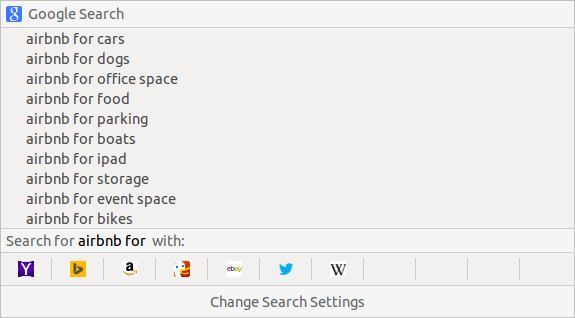
\includegraphics[width = \linewidth]{./images/airbnb_for_x.png} \\
  \begin{footnotesize}
  \emph{Notes}: This screenshot shows the Google ``auto-suggest'' query completions the phrase ``airbnb for'', which shows common queries entered by other users.
  This screenshot comes from the Google search toolbar in the Firefox browser, accessed on May 12, 2015.
  \end{footnotesize}
\end{minipage}
\end{figure} 

To move beyond the casual empiricism of considering what P2P rental markets might exist (or not) for various goods, we conducted a consumer survey on Amazon Mechanical Turk. 
The model and the survey complement each other in two ways. 
First, the survey helps justify some of the modeling conventions, such as making planned usage the primary explanation for the pattern of ownership rather than a taste for ownership or wealth. 
Second, the survey offers a partial decomposition of the BTM costs. 

\subsection{Main empirical results}
We find strong evidence that respondents who predicted that they would use a good more are more likely to own that good.
Increasing household income is associated with greater ownership, but even when controlling for income, predicted usage helps explain ownership. 
Among non-owners, planned usage was cited more often than a lack of income as the reason for non-ownership, with the exception of certain extremely expensive goods like vacation homes.
It may be the case that P2P rental markets might create more welfare in developing countries where individuals own fewer goods. 

The predictability of usage and the size of usage sessions for a good tend to be positively correlated.
In other words, goods that are used unpredictably tend to be used for relatively short periods.
These kinds of goods are also more likely to be owned. 
When we inspect goods that are the ``opposite''---predictable usage that ocurs in large chunks---we see goods that are often already rented in conventional markets.
These are also the goods where P2P rental markets seem to have had the most success.
Overall, we find that ownership and renting are gross substitutes, though there are notable outliers, such as the car, which is both widely owned and widely rented, presumably mostly because of trips that are initially take by plane. 

\subsection{Design and administration of the survey}
The survey focused on consumer decision-making and usage patterns for a variety of goods. 
Although MTurk offers a convenience sample, there is no strong reason to think its members would have highly idiosyncratic consumption patterns. 
Furthermore, for our purposes, the MTurk population is willing---and has incentives to---carefully answer a tedious set of questions.
Workers on MTurk who have their work ``rejected'' by dissatisfied employers become ineligible for the best, highest-paying kinds of work on the marketplace and therefore are diligent. 
This respondent diligence makes it useful for certain kinds of questions (for example, \cite{kuziemko2013elastic} used the MTurk population to study elasticities of demand for redistribution).  

We hired US-based ``Master'' workers to answer a questions about a consumer good, e.g., BBQ grill, pick-up truck, men's suit, canoe, etc.
We asked questions about a total of 26 goods that we selected because we thought they would yield interesting answers and varied in purpose (e.g., recreation, home improvement, cooking and so on), purchase price, predictability and usage size. 
We asked MTurk workers: whether they owned the good; whether they had ever rented or lent out the good; how much they would use the good \emph{regardless} of whether they actually owned the good; whether they would use the good in one large chunk, or in many small chunks; whether their usage was predictable; why they did not own the good; and finally, what was their household income. 
See Appendix~\ref{sec:survey} for the full list of goods as well as the actual survey questions and answers.  
Each ``human intelligence task'' or HIT comprised a total of eight questions about one particular good, with one question about family income. 
Workers were allowed to answer for each of the sampled goods.  

\subsection{Ownership by an individual's planned usage} 
In the model, consumers considered how much they would use some good and then compared the resultant usage utility against the purchase price. 
The model predicts increasing ownership in estimated usage.
Table~\ref{tab:ownership} shows that individuals reporting greater expected usage are more likely to own the good.
Furthermore, while higher household income predicts ownership, the strong association between expected usage and ownership persists even after taking income into account.

To elicit expected usage, we asked respondents to select how often they would use a good in time units, using familiar measures of time to label the responses e.g., 1 hour a week, 1 hour a day and so on.
We framed the choices as being approximately on a logarithmic scale, with each increase in usage being approximately a doubling of the fraction of time.
See Appendix~\ref{sec:survey} for the actual choices options and language.

Column~(1) of Table~\ref{tab:ownership} reports an OLS estimation of 
\begin{align} \label{eq:base_own}
\textsc{Own}_{ig} = \beta_0 + \beta_1 \log x_{ig} + c_{g} + \epsilon_{g}, 
\end{align}
where $\textsc{Own}_{ig}$ takes the value of $1$ if respondent $i$ reported owning good $g$, otherwise $0$, $x_{ig}$ is their reported fraction of time they estimate they would spend using the good and $c_g$ is a good-specific fixed effect.
Standard errors are clustered at the level of the good. 
In Column~(2), a control for log family income is included while in Column~(3), a respondent fixed effect is added. 


% Table created by stargazer v.5.1 by Marek Hlavac, Harvard University. E-mail: hlavac at fas.harvard.edu
% Date and time: Thu, May 14, 2015 - 07:55:45 AM
% Requires LaTeX packages: dcolumn 
\begin{table}[!htbp] \centering 
  \caption{Respondent estimates of the fraction of time spent using a good and whether they own that good} 
  \label{tab:ownership} 
\footnotesize 
\begin{tabular}{@{\extracolsep{5pt}}lD{.}{.}{-3} D{.}{.}{-3} D{.}{.}{-3} } 
\\[-1.8ex]\hline 
\hline \\[-1.8ex] 
 & \multicolumn{3}{c}{\textit{Dependent variable:}} \\ 
\cline{2-4} 
\\[-1.8ex] & \multicolumn{3}{c}{Respondent owns the item?, ($\textsc{Own}_{ig}=1$)} \\ 
\\[-1.8ex] & \multicolumn{1}{c}{(1)} & \multicolumn{1}{c}{(2)} & \multicolumn{1}{c}{(3)}\\ 
\hline \\[-1.8ex] 
 Log estimated usage, $\log x_{ig}$ & 0.026^{**} & 0.026^{**} & 0.026^{**} \\ 
  & (0.011) & (0.011) & (0.011) \\ 
  Log household income, $\log y_i$ &  & 0.102^{***} &  \\ 
  &  & (0.025) &  \\ 
 \hline \\[-1.8ex] 
Good FE & \multicolumn{1}{c}{Y} & \multicolumn{1}{c}{Y} & \multicolumn{1}{c}{Y} \\ 
Respondent FE & \multicolumn{1}{c}{N} & \multicolumn{1}{c}{N} & \multicolumn{1}{c}{Y} \\ 
Observations & \multicolumn{1}{c}{411} & \multicolumn{1}{c}{411} & \multicolumn{1}{c}{411} \\ 
R$^{2}$ & \multicolumn{1}{c}{0.445} & \multicolumn{1}{c}{0.465} & \multicolumn{1}{c}{0.567} \\ 
\hline 
\hline \\[-1.8ex] 
\end{tabular}
\\{\footnotesize \begin{minipage}{0.75 \linewidth} \emph{Notes:}
This table reports OLS regressions where the dependent variable is an indicator for whether a respondent reported owning a particular good.
In Column~(1) the independent variable is that respondent's estimate of what fraction of their time they would spend using that good (in logs).
In Column~(2) a regressor for the log of the respondent's self-reported household income is added to the Column~(1) specification.
Column~(3) uses the same specification as Column~(1), but a respondent specific fixed effect is added. 
The sample is restricted to respondents who reports some positive amount of predicted usage of the good and reported their household income.
All regressions include good-specific fixed effects and standard errors are clustered at the good level. 
\starlanguage \end{minipage} }
\end{table}


As the model predicts, higher estimated usage is associated with ownership.
The coefficient on the estimated usage regressor in Column~(1) implies that a doubling of expected usage for some good---say using a BBQ grill two hours a week instead of one hour---is associated with about a 2.5 percentage point increase in probability of ownership. 
In Column~(2), the coefficient on the usage regressor is the same magnitude, despite the inclusion of log of self-reported household income (in thousands) in the specification.\footnote{
  Household incomes imputed by taking the midpoint of the range associated with each bin (i.e., a respondent's selecting \$10,000-\$19,999 are imputed to have a \$15K family income).
  There was only one top-coded respondent and they were given an imputed income of 1.5 times the censoring threshold.
  See Appendix~\ref{sec:survey} for the actual income bands respondents could select from.
  }
As we would expect given that most of the goods listed are normal, a higher income is associated with greater probability of ownership---a 10\% increase in household income is associated with a 1\% increase in the probability of ownership.  
However, the lack of change in the usage regressor implies that the pattern found in Column~(1) is not simply the result of higher income respondents being more likely to own and to report greater expected usage generally (perhaps because of greater leisure time). 
In Column~(3) we re-estimate Column~(1) but include respondent-specific fixed effects as well.
As with the other specifications, the the strong positive relationship between expected usage and ownership persists. 

\subsection{Self-reported reasons for non-ownership}

The regression results from the previous section suggest that both income and predicted usage are important for explaining the ownership decision. 
These two factors are presumably more or less important for different kinds of goods.
Figure~\ref{fig:reasons} shows that there is in substantial good-level heterogeneity in the reported reasons of non-owners.
However, for the goods we surveyed, explanations for non-ownership are strongly tilted towards usage considerations rather than income considerations.

\begin{figure}
\centering 
\caption{Fraction of non-owners citing usage versus fraction citing income as the reason for ownership decision} 
\label{fig:reasons}
\begin{minipage}{0.60 \linewidth}
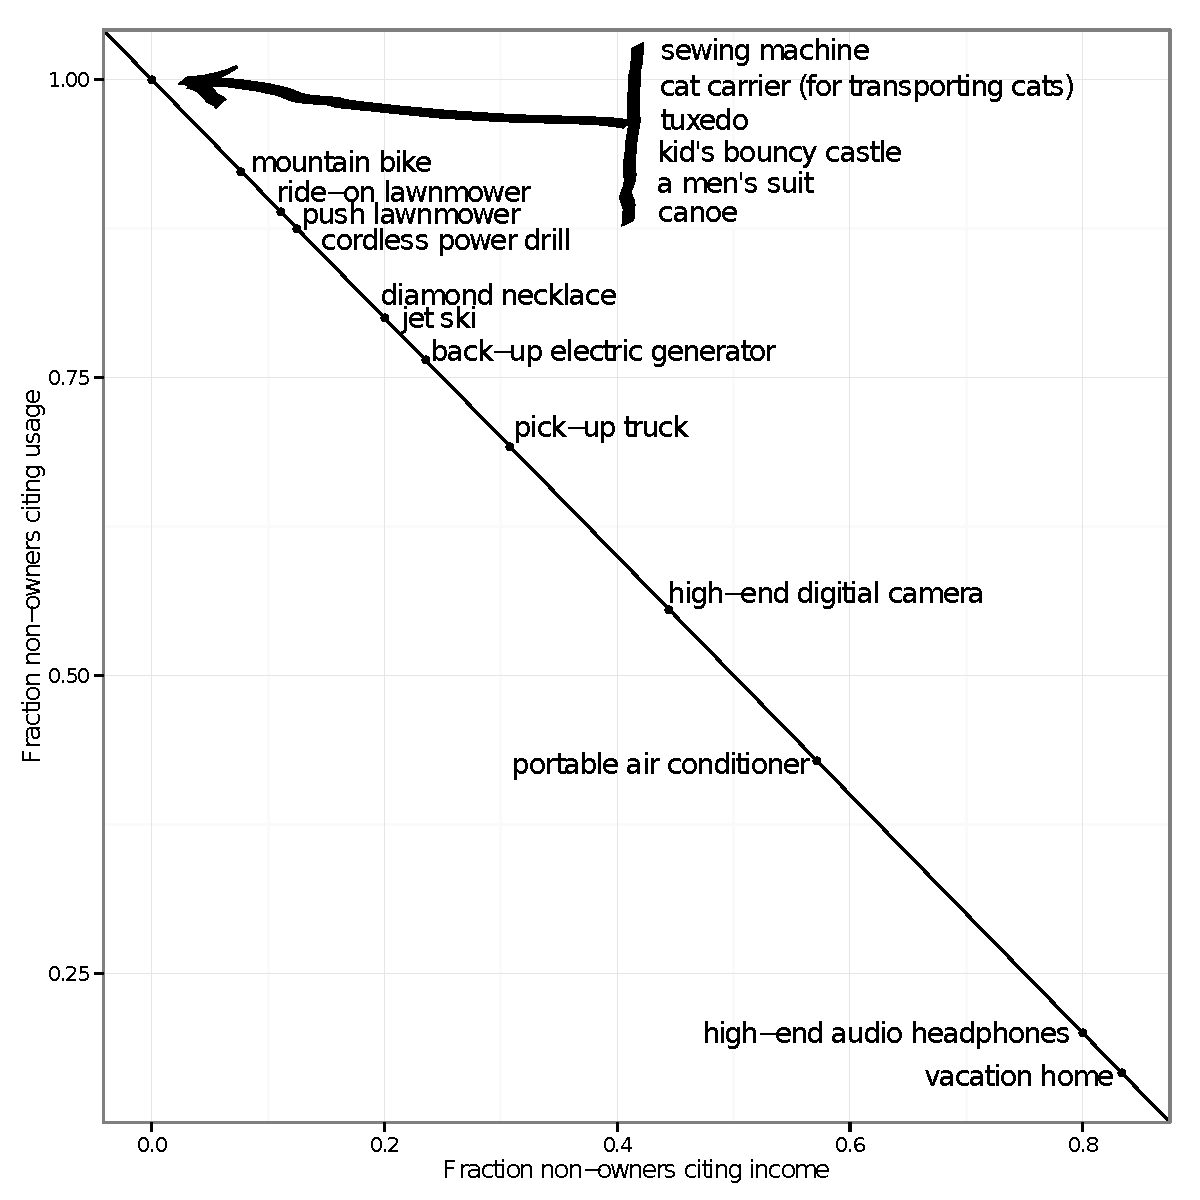
\includegraphics[width = \linewidth]{./plots/reasons_for_nonownership.pdf} 
\end{minipage} 
\end{figure} 

Non-owners were asked for the primary reason for not-owning and good and could cite usage (``We wouldn't use it enough to justify the purchase price''), income  (``We would use it, but we simply do not have the money'') or space (``We don't have space for this item.'').
Space was not frequently cited and so in Figure~\ref{fig:reasons} we plot the per-good fractions citing usage versus income, among those that cited either income or usage and for which the good in question had seven or more non-owners. 
There are some goods for which income was not cited at all (e.g., sewing machine, tuxedo, canoe), and several others where usage was overwhelming more likely to be cited.
The only goods where a larger fraction of respondents cited income than cited usage was high-end headphones and vacation homes. 

\subsection{Aggregate usage chunkiness and predictability} 

Two major practical determinants of how feasible a rental market are the predictability and size of usage sessions. 
Goods where it is easy to predict when they will be needed (perhaps because it is easy for the owner to choose when to use the good with little loss in utility) would be easier to rent (or lend out).
In contrast, goods that have inherently unpredictable usage or goods where there is little flexibility in when they are used would be difficult to rent out without substantial utility loss to the owner.
Similarly, for goods that are used in numerous small sessions, renting or lending out the good to others would create high transaction costs.

We asked subjects about the predictability and chunkiness of their usage for the goods and found that these measures strongly covary (with some exceptions, which we will discuss):
the smaller chunk of typical usage, the more unpredictable the usage is.
For example, respondents rated a hammer as being used in small chunks of time (say when hanging a picture) and this usage is unpredictable. 
In contrast, a tuxedo scores low on both measures---it is used for a substantial amount of time (say when attending a wedding) and that usage can be predicted far in advance.  

\begin{figure}
\centering 
\caption{Usage predictability versus chunkiness \label{fig:granularity_v_predictability}}
\begin{minipage}{0.60 \linewidth}
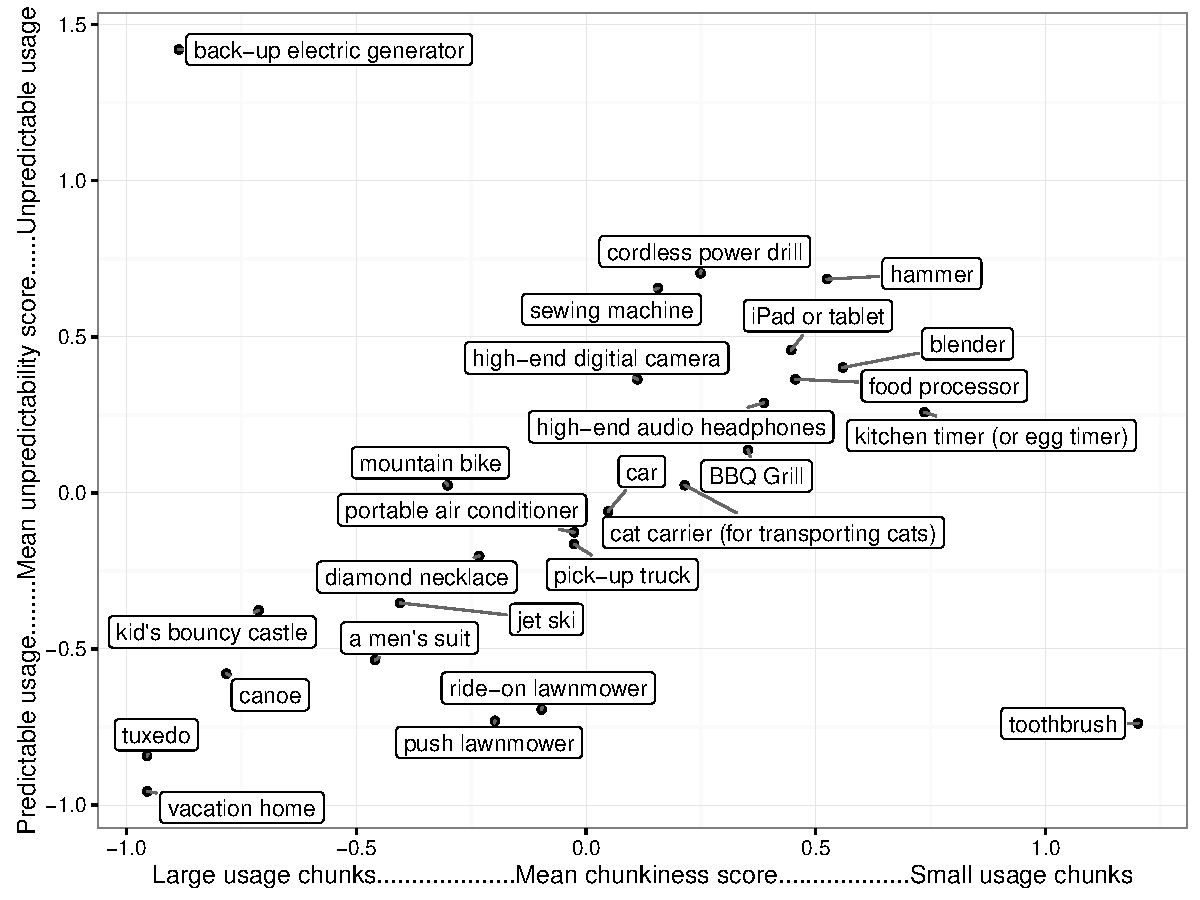
\includegraphics[width = \linewidth]{./plots/granularity_versus_predictability.pdf} 
\emph{Notes:} Scatter plot showing mean predictability versus chunkiness. 
\end{minipage} 
\end{figure} 

For each good, respondents were asked to rate the unpredictability of usage on a 1-5 scale (1 was highly predictable and 5 was highly unpredictable) as well as chunkiness (1 was one big chunk--- and 5 was low chunkiness---lots of little chunks).  
Figure~\ref{fig:granularity_v_predictability} plots the mean unpredictability score against the mean chunkiness score. 
It shows a strong relationship between chunkiness and predictability, with two notable outliers: the toothbrush and the generator. 
A toothbrush is used in small chunks (2 minutes according to the ADA) and its usage is highly predictable (after every meal, according to the ADA).
The back-up electric generator is the toothbrush's opposite---power can go out for days or even weeks during a disaster and this event is rarely predictable. 
These common-sense answers are not particularly illuminating but they do show subjects were paying attention and offering reasonable answers. 

If we examine goods near the origin, we see goods well-suited to rental, in that they have predictable usage that occurs in large chunks. 
Not surprisingly, these are often goods for which conventional rental markets already exist---formal wear (tuxedos), vacation homes, sporting equipment (canoes and jet skis for rent at lakes) and so on.
As we move a bit further, from the origin, we see goods for which there is not much of a rental market (bikes, lawnmowers, jewelry) but would seem to have the attributes necessary to support such a market, assuming there are in fact enough non-owners to support such a market.  

\subsection{Chunkiness, predictability and ownership} 

We test whether the predictability and chunkiness measures are related to individual ownership. 
Table~\ref{tab:ownership_attr} shows that they are, in the expected direction:
\important{goods with unpredicatable usage that occurs in small chunks are substantially more likely to be owned.}
Furthermore, it is not the case that these two measures are simply capturing some single latent ``rentability'' measure, as each seems to have an independent effect on the probability of ownership. 


% Table created by stargazer v.5.2 by Marek Hlavac, Harvard University. E-mail: hlavac at fas.harvard.edu
% Date and time: Tue, Jan 26, 2016 - 07:25:30 AM
% Requires LaTeX packages: dcolumn 
\begin{table}[!htbp] \centering 
  \caption{Good usage unpredictability and chunkiness and its association with good ownership.} 
  \label{tab:ownership_attr} 
\footnotesize 
\begin{tabular}{@{\extracolsep{5pt}}lD{.}{.}{-3} D{.}{.}{-3} D{.}{.}{-3} D{.}{.}{-3} } 
\\[-1.8ex]\hline 
\hline \\[-1.8ex] 
 & \multicolumn{4}{c}{\textit{Dependent variable:}} \\ 
\cline{2-5} 
\\[-1.8ex] & \multicolumn{4}{c}{Item is owned} \\ 
\\[-1.8ex] & \multicolumn{1}{c}{(1)} & \multicolumn{1}{c}{(2)} & \multicolumn{1}{c}{(3)} & \multicolumn{1}{c}{(4)}\\ 
\hline \\[-1.8ex] 
 Unpredictability Score (US) & 0.139^{***} &  & 0.095^{***} & 0.003 \\ 
  & (0.030) &  & (0.034) & (0.034) \\ 
  Chunkiness Score (CS) &  & 0.135^{***} & 0.091^{***} & -0.018 \\ 
  &  & (0.025) & (0.029) & (0.025) \\ 
  US x CS &  &  & -0.009 & 0.006 \\ 
  &  &  & (0.018) & (0.018) \\ 
 \hline \\[-1.8ex] 
Respondent FE & \multicolumn{1}{c}{Y} & \multicolumn{1}{c}{Y} & \multicolumn{1}{c}{Y} & \multicolumn{1}{c}{Y} \\ 
Good FE & \multicolumn{1}{c}{N} & \multicolumn{1}{c}{N} & \multicolumn{1}{c}{N} & \multicolumn{1}{c}{Y} \\ 
Observations & \multicolumn{1}{c}{489} & \multicolumn{1}{c}{489} & \multicolumn{1}{c}{489} & \multicolumn{1}{c}{489} \\ 
R$^{2}$ & \multicolumn{1}{c}{0.170} & \multicolumn{1}{c}{0.169} & \multicolumn{1}{c}{0.191} & \multicolumn{1}{c}{0.500} \\ 
\hline 
\hline \\[-1.8ex] 
\end{tabular}
\\ {\footnotesize  \begin{minipage}{0.85 \linewidth} \emph{Notes:}
This table reports regressions of an indicator for whether the respondent owns a good on that same respondent's estimates of the unpredictability and granularity of usage for that good.
The two indices are normalized responses to the 1-5 scale questions on usage chunkiness and unpredictability, pooled over all respondents and goods.
Toothbrushes and backup generators are excluded from the sample. 
See Appendix~\ref{sec:survey} for the actual survey language and responses.
In each regression, a respondent-specific fixed effect is included.
Standard errors are clustered at the level of the individual respondent.
\starlanguage
\end{minipage} }
\end{table}
 

Column~(1) of Table~\ref{tab:ownership_attr} reports an estimate of 
\begin{align}
  \text{Own}_{ig} = \beta_0 + \beta_1 \textsc{UnpredictabilityScore}_{ig} + c_i + \epsilon_i
\end{align} 
where $\textsc{UnpredictabilityScore}_{ig}$ is the normalized predictability score for good $g$ by respondent $i$.
The coefficient on the unpredictability score is positive and highly significant, with a one standard deviation decrease in predictability increasing the probability of ownership by about 14 percentage points. 
In Column~(2) we instead use the chunkiness measure as the predictor and also find a positive and highly significant effect of about the same magnitude. 
In Column~(3) we interact the the chunkiness and predictability measures.
Each measure has a slightly smaller effect (though a formal hypothesis test would fail to reject a difference relative to the estimate when each measure appeared alone); their interaction term, while negative, is small and far from significant.

One concern with our approach might be that respondents prone to reporting high or low chunkiness and predictability scores might be idiosyncratically more or less likely to own the good.
In other words, the patterns from Columns~(1) through (3) might reflect individual differences rather than general attributes about the good.
In Column~(4) we use the same specification as Column~(3) but include a good-specific effect.
With this effect, the coefficients on all regressors end up close to zero, which supports the notion that the patterns in the previous regressions really are driven by the nature of the good. 

\subsection{Aggregate ownership and renting patterns at the level of the good}

This paper was motivated by the fact that P2P rental markets have \emph{begun} to flourish.
Thus, asking respondents whether they have rented a particular good in a P2P rental market would likely yield uninteresting results, given how new these markets are.
However, the existing P2P rental market platforms seem to be focusing on sectors where conventional rental markets already existed (or at least met the same want, say in the case of Airbnb offering a substitute for hotels).
As such, asking respondents if they have ever rented a good at all might be a reasonably proxy for whether they would eventually rent such a good in a P2P rental market. 
For each good, we asked whether the respondent's household (a) owned the good and (b) had ever rented the good.
As Figure~\ref{fig:scatter} will show, renting and owning are gross substitutes in the data, when cars are excluded.
Cars show a high level of both ownership and rental. 

\begin{figure}
\centering 
\caption{Fraction renting versus fraction owning \label{fig:scatter} }
\begin{minipage}{0.60 \linewidth}
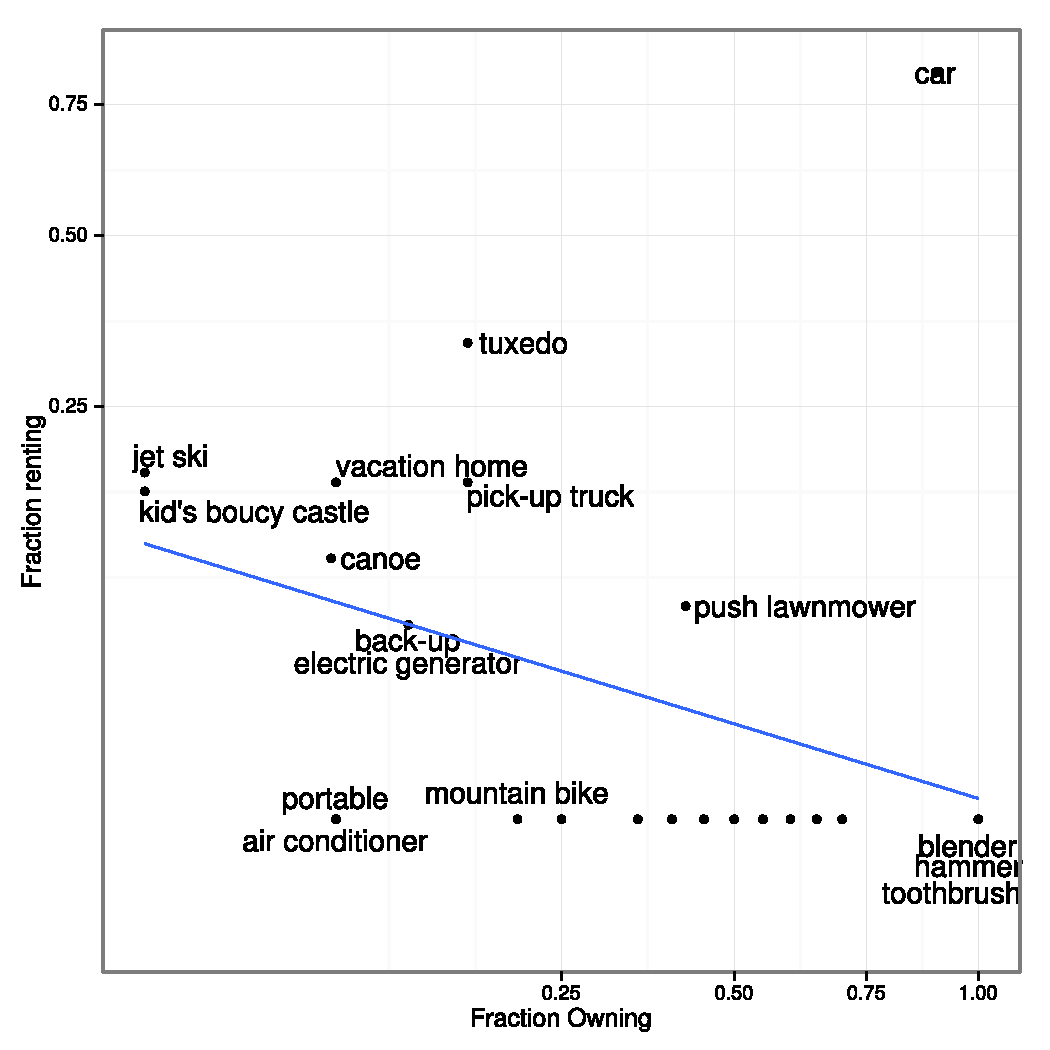
\includegraphics[width = \linewidth]{./plots/scatter_rent_v_own.pdf} 
\end{minipage} 
\end{figure} 

In Figure~\ref{fig:scatter}, the fraction owning is plotted on the x-axis and the fraction renting on the y-axis.
Both axes are on a log scale. 
Some notable goods are labeled---see Appendix~\ref{sec:additional_results} for the precise by-good fractions for every good.

Unsurprisingly, goods with nearly universal ownership show little renting. 
There are a number of goods (not all labeled) that show medium ownership levels (e.g., around 50\%) and yet zero recorded instances of renting, which could indicate potential P2P rental market candidates. 
Goods that are used during special occasions like weddings, celebrations and vacations show the highest rates of rental and lowest rates of ownership, e.g., tuxedos, vacation homes, jet ski, tuxedos, canoes, bouncy castles. 


% Table created by stargazer v.5.2 by Marek Hlavac, Harvard University. E-mail: hlavac at fas.harvard.edu
% Date and time: Tue, Jan 26, 2016 - 07:25:21 AM
% Requires LaTeX packages: dcolumn 
\begin{table}[!htbp] \centering 
  \caption{Fraction of respondents owning a good versus fraction having rented a good} 
  \label{tab:own_vs_rent} 
\footnotesize 
\begin{tabular}{@{\extracolsep{5pt}}lD{.}{.}{-3} D{.}{.}{-3} } 
\\[-1.8ex]\hline 
\hline \\[-1.8ex] 
 & \multicolumn{2}{c}{\textit{Dependent variable:}} \\ 
\cline{2-3} 
\\[-1.8ex] & \multicolumn{2}{c}{Fraction reporting renting the good (\textsc{FracRental})} \\ 
\\[-1.8ex] & \multicolumn{1}{c}{(1)} & \multicolumn{1}{c}{(2)}\\ 
\hline \\[-1.8ex] 
 Fraction reporting owning the good & -0.009 & -0.160^{***} \\ 
  & (0.109) & (0.046) \\ 
  Constant & 0.081 & 0.115^{***} \\ 
  & (0.059) & (0.024) \\ 
 \hline \\[-1.8ex] 
Sample & \multicolumn{1}{c}{All Goods} & \multicolumn{1}{c}{Cars Excluded} \\ 
Observations & \multicolumn{1}{c}{26} & \multicolumn{1}{c}{25} \\ 
R$^{2}$ & \multicolumn{1}{c}{0.0003} & \multicolumn{1}{c}{0.345} \\ 
\hline 
\hline \\[-1.8ex] 
\end{tabular}
\\{\footnotesize \begin{minipage}{0.85 \linewidth} \emph{Notes:}
The unit of observation for the regressions in this table is the individual good.
The dependent variable is the fraction of respondents reporting having rented that good, while the independent variable is the fraction reporting owning that good. 
Column~(1) includes all goods surveyed, while Column~(2) excludes cars.
For the full list of goods and the survey language, see Appendix~\ref{sec:survey}. 
\starlanguage \end{minipage} }
\end{table}


To confirm the visual pattern of renting declining in ownership, Column~(1) of Table~\ref{tab:own_vs_rent} reports an estimate of 
\begin{align}
\textsc{FracRent}_g = \beta_0 + \beta_1 \textsc{FracOwn}_g + \epsilon,  
\end{align} 
where $\textsc{FracOwn}_g$ is the fraction of respondents claiming to own good $g$ and $\textsc{FracRent}_g$ is the fraction claiming to have rented good $g$.
Column~(1) reports the estimated regression of this equation with cars, while in Column~(2), cars are excluded.
If we exclude cars, there is a strong negative relationship between owning and renting;
a 10\% increase in the fraction owning reduces the fraction of households renting by a little more than 1.5 percentage points. 

\section{Conclusion} 

One area where P2P rental markets could have a long-term effect is on the diversity of goods consumed. 
Consider that in some formulations of the consumer problem, consumers consume some positive amount of every good offered.
This is obviously a large departure from empirical reality if we draw fine-grained distinctions among ``goods.'' 
For example, Amazon.com currently lists 6,238 results for ``blender'' in the Home \& Kitchen category: 
presumably most households own far fewer than this, with most owning one or none.\footnote{As of October 8th, 2014.}
The reason for this pattern in the language of this model is clear: 
a consumer's $\alpha$ for Blender 2 \emph{conditional} upon owning Blender 1 is quite low and so a second blender is not purchased.
However, if a rental market existed for both blender types, consumers could act upon their taste for diversity without owning a dozen blenders. 
Even if the blender example seems implausible, we should consider that very few consumers try to rent the car when on vacation that they normally drive in their hometown. 
Presumably they diversify consumption in these cases precisely because it is easy to. 

One long-term reaction to the rising of P2P rental markets is that firms might change the goods that they offer. 
As P2P rental markets become commonplace, manufacturers will begin designing products that cater to this additional purpose. 
For example, locks on cars and houses that allow remote entry will be more appealing. 
The emerging Internet-of-Things will make it easier to identify goods that are not being used at a moment in time and perhaps facilitate trade automatically.
If autonomous vehicles and drones become commonplace, even the seemingly unavoidable transaction costs associated with moving goods to where they are needed might be substantiall diminished.\footnote{Thanks to Jonathan Hall for making this point.}
Similarly, technologies that make it easier to monitor usage (GPS, embedded sensors, streaming video of how they are being used and so on) should make contracting easier and reduce some of the informational asymmetries that contribute to transaction costs. 
As more of economic and social life are computer-mediated, platforms will use this information to verify the identify and reputation of buyers and sellers, further mitigating moral hazard and adverse selection.  

Our model makes several predictions that are---or should become---testable over time, as P2P rental markets grow.
Some obvious candidates include examining whether the emergence of P2P rental markets increase access by non-owners, changes the ownership decision and affects rental rates.
Given the substantial legal and regulatory obstacles many sharing economy companies face---including being banned in some places at certain periods of time---might make credible quasi-experimental designs feasible. 

% \cite{ikkala2014defining}

\bibliographystyle{aer}
\bibliography{sharing.bib}

\newpage 

\appendix 

\section{Survey Questions \label{sec:survey}} 

The actual goods were: 

\begin{itemize} 
\item BBQ Grill
\item toothbrush
\item a men's suit
\item blender
\item canoe
\item car
\item cordless power drill
\item hammer
\item diamond necklace
\item food processor
\item hammer
\item cat carrier (for transporting cats)
\item high-end audio headphones
\item high-end digitial [sic] camera
\item iPad or tablet
\item jet ski
\item kid's boucy [sic] castle
\item kitchen timer (or egg timer)
\item mountain bike
\item pick-up truck
\item push lawnmower
\item ride-on lawnmower
\item tuxedo
 \item vacation home
\item back-up electric generator
\item portable air conditioner
\item sewing machine
\end{itemize} 

\begin{itemize} 

\item Does your household own a {\bf good}?
\begin{itemize}
\item Yes
\item No
\end{itemize} 

\item Have you ever lent your {\bf good} to someone else?
\begin{itemize}
\item Yes
\item No
\item NA - we do not own one.
\end{itemize} 

\item Have you ever borrowed a {\bf good} from someone else?
\begin{itemize}
\item Yes
\item No
\item NA - we own one.
\end{itemize} 

\item Have you ever rented a {\bf good}?
\begin{itemize}
\item Yes
\item No
\item NA - we own one.
\end{itemize} 

\item Regardless of whether your household owns a {\bf good}, if you did own one, how much do you estimate it would be used by members of your household on average?

\begin{itemize} 
\item We would not use this at all
\item 1 minute a week (about 1 hour a year) 
\item 5 minutes a week (about 4 hours a year)
\item 1/2 an hour a week
\item 1 hour a week
\item 1/2 an hour a day
\item 1 hour a day
\item 2 hours a day
\item 4 hours a day
\item 8 hours a day
\item 16 hours a day
\item 24 hours a day (I would continuously be using this good)
\end{itemize} 

\item Regardless of whether you actually own a {\bf good}, how do you imagine it would be used if it was owned by your household (on a scale of 1 to 5): 
\begin{itemize} 
\item 1 - Used in one big block of time
\item 2  
\item 3 - Used in a mixture of large and small blocks of time
\item 4 
\item 5 - Used in many small blocks of time
\end{itemize} 

\item Regardless of whether you actually own a {\bf good}, how predictable would your usage of it be if you did own it: 
\begin{itemize}
\item 1 - Very predictable---I can plan usage many weeks in advance
\item 2  
\item 3 - Somewhat predictable 
\item 4 
\item 5 - Very unpredictable---I would never know exactly when I would need to use it until right beforehand. 
\end{itemize} 

\item If you do not own a {\bf good}, what is the primary reason?
\begin{itemize} 
\item NA - we own one.
\item We wouldn't use it enough to justify the purchase price
\item We would use it, but we simply do not have the money.
\item I don't have the space for this item
\end{itemize} 

\item What is your total household income? 
\begin{itemize} 
\item Less than \$10,000
\item  \$10,000-\$19,999
\item  \$20,000-\$29,999
\item  \$30,000-\$39,999
\item  \$40,000-\$49,999
\item  \$50,000-\$59,999
\item  \$60,000-\$69,999
\item  \$70,000-\$79,999
\item  \$80,000-\$89,999
\item  \$90,000-\$99,999
\item  \$100,000-\$149,000
\item  More than \$150,000
\end{itemize} 

\end{itemize}

\section{Additional empirical results} \label{sec:additional_results}

Figure~\ref{fig:frac_owning} shows the fraction of respondents reporting owning various goods, as well as 95\% confidence intervals for that point estimate computing using the Wilson method for a binary proportion.    
There are few surprises: nearly everyone owns a toothbrush, a hammer and a blender; no one reported owning a jet ski and only one respondent reported owning a vacation home.
Figure~\ref{fig:frac_renting} shows the fraction of respondents reporting having rented the various goods. 
\important{Generally, ownership and renting appear to be gross substitutes, with the notable exception of cars, presumably because people rent cars when traveling.}

\begin{figure}
\centering 
\caption{Fraction of respondents owning various goods \label{fig:frac_owning} }
\begin{minipage}{0.90 \linewidth}
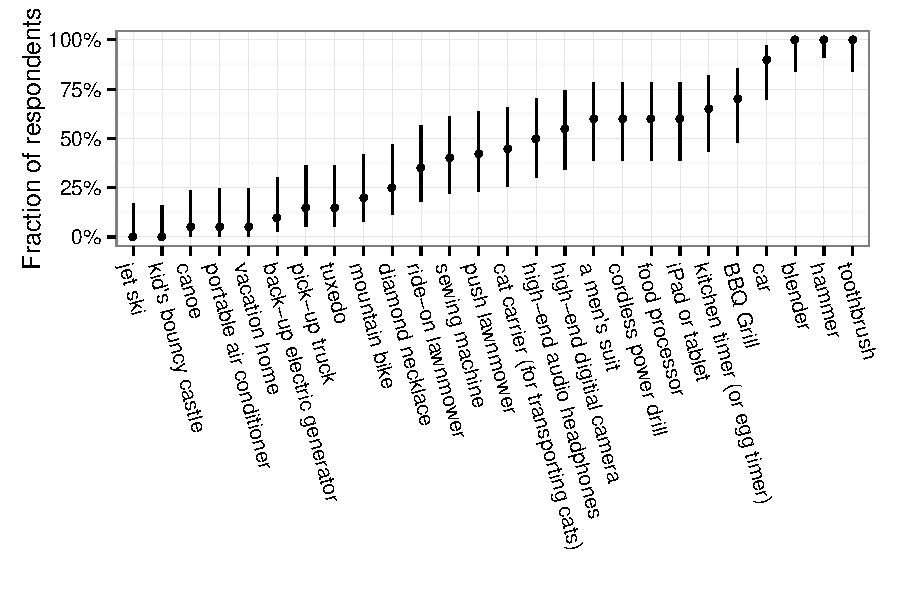
\includegraphics[width = \linewidth]{./plots/ownership_fractions.pdf} 
\end{minipage} 
\end{figure} 

\begin{figure}
\centering 
\caption{Fraction of respondents reporting having rented various goods \label{fig:frac_renting}}
\begin{minipage}{0.90 \linewidth}
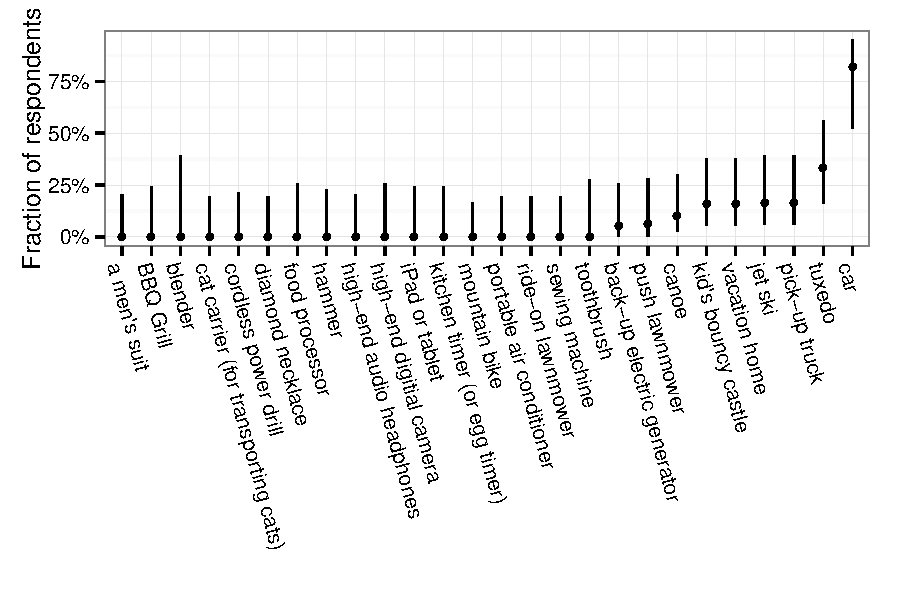
\includegraphics[width = \linewidth]{./plots/rental_fractions.pdf} 
\end{minipage} 
\end{figure} 

The mean unpredictability scores by good seem sensible: 
Figure~\ref{fig:predict_index} shows the mean unpredictability index per good. 
The most predictable goods are either those associated with planned recreation (e.g., vacation home, canoe, jet ski, tuxedo) or predictable chores (e.g., toothbrush, the two kinds of lawnmowers). 
The most unpredictable goods are associated with either food preparation (e.g., blender, food processor) or repairs (e.g., hammer, sewing machine, cordless power drill). 
Back-up electric generator is a clear (and unsurprising) outlier---you are in a sense always ``surprised'' when you need to use it. 


\begin{figure}
\centering 
\caption{Mean unpredictability index by good \label{fig:predict_index} }
\begin{minipage}{0.90 \linewidth}
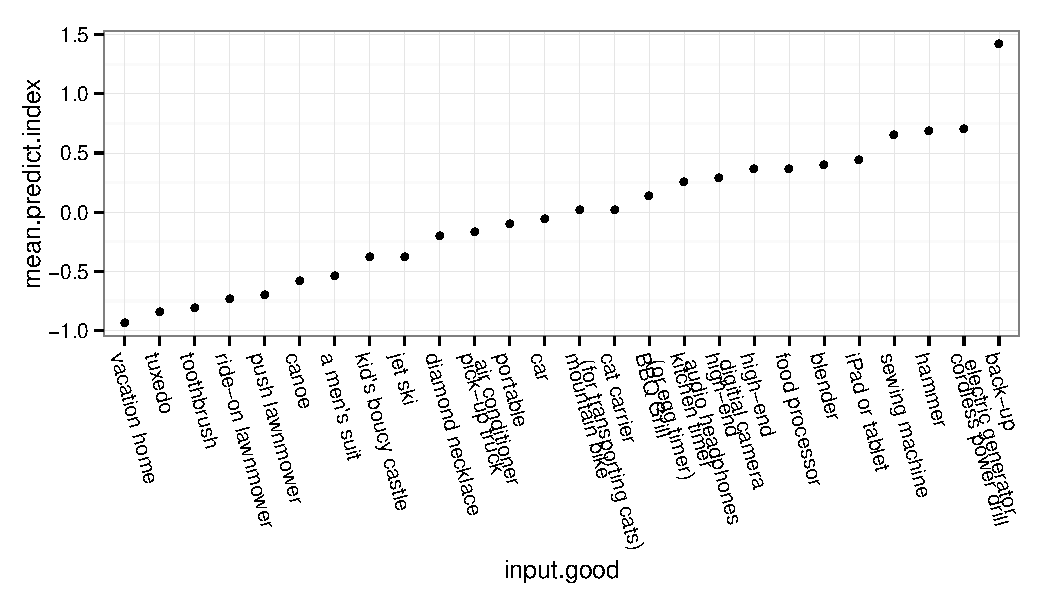
\includegraphics[width = \linewidth]{./plots/predictability.pdf} 
\end{minipage} 
\end{figure} 

Figure~\ref{fig:granularity} shows the mean chunkiness index per good. 
There appears to be some similarity in high predictable usage, but some goods used in small chunks of time also appear to have highly predictable usage---namely the toothbrush. 
To make this relationship explicit, in Figure~\ref{fig:granularity_v_predictability} the chunkiness and predictability indices are plotted against each other. 
\important{With the exception of two goods---the toothbrush and back-up generator---predictability and chunkiness are strongly positively correlated.}

\begin{figure}
\centering 
\caption{Mean chunkiness index by good \label{fig:granularity}}
\begin{minipage}{0.90 \linewidth}
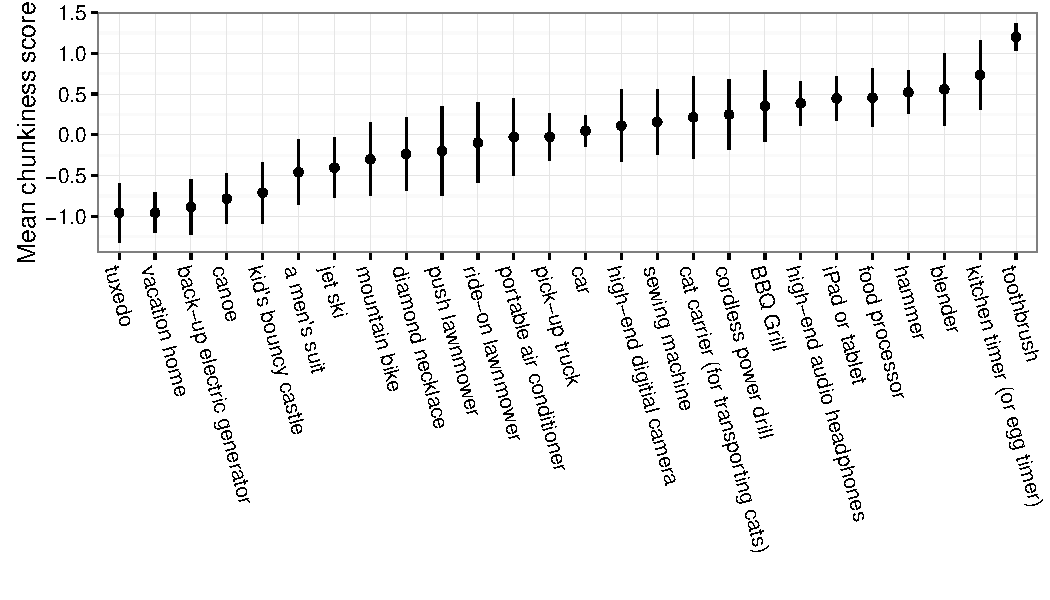
\includegraphics[width = \linewidth]{./plots/granularity.pdf} 
\end{minipage} 
\end{figure} 

\end{document} 

\section{New New Stochastic Model}

A would-be-user of some good learns their valuation from using that good that period.
That value is $v \sim U[0,1]$.
The owner always has the outside option $\underline{u}$ of using some other good. 
If $v > \underline{u}$, the use the good, otherwise they do not.
The realized utility from owning the good is thus:
\begin{align}
  \int_{\underline{u}}^1 v dv = \frac{1}{2} - \frac{\underline{u}^2}{2}
\end{align} 
This determines their purchase decision---if the pro-rated purchase price is less than the utility, then they buy, otherwise they do not.
Assume that a fraction of consumers $\theta$ own the good and $(1-\theta)$ do not. 

The owners of the good can rent to the non-owners at a market-clearing rental rate of $r$, after paying a transaction cost of $c$. 
We first note that if $c > r$, then no owner chooses to rent out the good and there would be no supply to the market.
For $r - c > 0$, the owner would be willing to rent some of the time.
For $r - c < \underline{u}$, the owner would simply rent out during periods when they would not have used the good anyway.
This occurs $\underline{u}$ of the time and so the market supply would simply be $\underline{u}\theta$.
For a sufficiently high rental rate, the owner would also economize of their usage, renting out during some relatively low-value periods when they otherwise would have consumed.
For $r - c > \underline{u}$, market supply is $\theta (r - c)$.
The supply curve (plotted in Figure~\ref{fig:supply}) is 
\begin{align}
S(r) =  \left\{
     \begin{array}{ll}
       0                       & : 0 > r - c  \\
       \theta \underline{u}    & : 0 < r - c < \underline{u} \\ 
       \theta (r - c)          & : \underline{u} < r - c   
     \end{array}
   \right. 
\end{align} 

\begin{figure}
\centering 
\caption{Short-run P2P rental market supply curve}
\label{fig:supply} 
\begin{minipage}{0.50 \linewidth}
  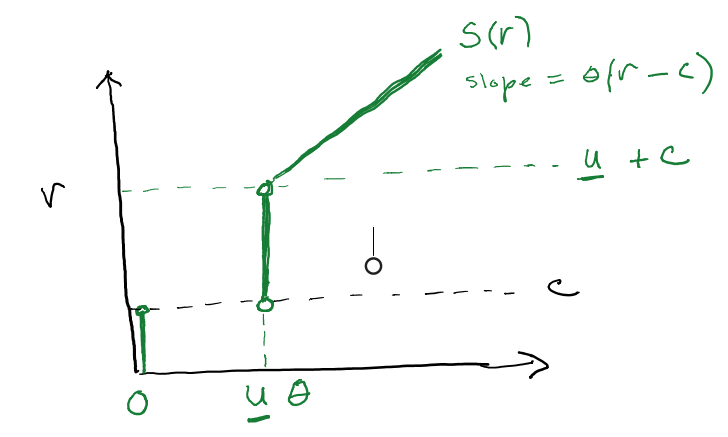
\includegraphics[width = \linewidth]{./figures/supply_curve.png} \\
  \begin{footnotesize}
  \emph{Notes}: Here is a supply curve. 
  \end{footnotesize}
\end{minipage}
\end{figure} 

On the demand side, a non-owner is willing to rent if $v - r > \underline{u}^R$, where $\underline{u}^R$ is the outside option of non-owners.
The demand curve is thus
\begin{align} 
D(r) =  \left\{
\begin{array}{ll}
      (1 - \theta) ( 1- \underline{u}^R)   & : r < \underline{u}^R \\
      (1 - \theta) (1 - r)            & : r > \underline{u}^R 
     \end{array}
   \right. 
\end{align} 

\begin{figure}
\centering 
\caption{Short-run P2P rental market demand curve}
\label{fig:demand} 
\begin{minipage}{0.50 \linewidth}
  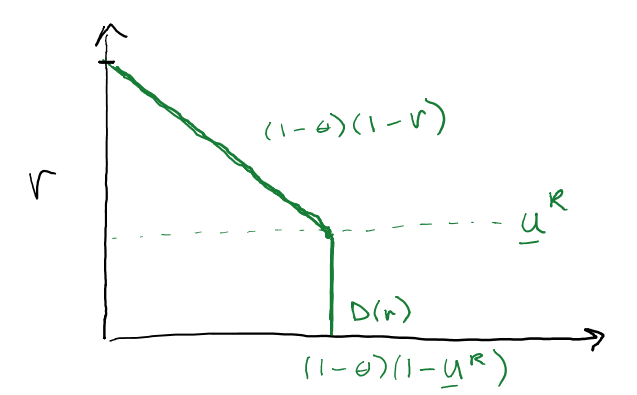
\includegraphics[width = \linewidth]{./figures/demand_curve.png} \\
  \begin{footnotesize}
  \emph{Notes}: Here is a demand curve. 
  \end{footnotesize}
\end{minipage}
\end{figure} 

\subsection{Equilibrium}
There are several possibile equilibria.
TK - NOTE: I have not worked out the conditions under which these different equilibrium arise.
Not all might be possible, especially if we assume (reasonably) that $\underline{u} < \underline{u}^R$. 

\paragraph{No trade equilibrium} 
If $c$ is sufficiently high, then the good is not transacted at all.
This would occur if $c > 1$, as $v = 1$ is the highest possible valuation a non-owner can have for the good.

\paragraph{``Owners consume the same'' equilibrium}
There is an equilibrium where the vertical portion of the supply curve---where only unused capacity is sold---intersects the sloping portion of the demand curve, or $\theta \underline{u} = (1 - \theta)(1 - r)$, 
which gives a market-clearing rental rate of
\begin{align}
  r = 1 - \underline{u} \left( \frac{\theta}{1 - \theta} \right).
\end{align} 
As we would expect, as the relative number of owners increases, rental rates fall.
The higher the value of $\underline{u}$, the greater the fraction of time owners would not have used the good anyway, and hence the greater supply and lower rental rates.

\paragraph{``Owners and non-owners economize on usage'' equilibrium} 
There is an equilibrium where sloping portions of the two curves intersect, giving a market-clearing rental rate of
\begin{align}
  r = 1 - \theta(1 - c).
\end{align} 
As transaction costs rise, the rental rate increases.
As expected, more owners lowers the rental rate, as this increases supply on the market. 

\paragraph{``Owners economize but non-owners do not'' equilibrium} 
In this equilibrium, the sloping portion of the supply curve intersects the vertical portion of the demand curve, giving an equilibrium rental rate of 
\begin{align}
  r = c + \left( \frac{1 - \theta}{\theta } \right) (1 - \underline{u}^R)
\end{align} 

When $\underline{u}^R$ is goes up, there is less demand and so rental rates fall.
Rental rates are increasing in the transaction costs.
The greater the relative number of non-owners, the higher the rental rate.


\section{New stochastic model} 
In each period, a consumer would get some value from using a good with probability $q$. 
If they want to use the good, they would get a value $v \sim U(0, 1]$. 
The outside option of not using the good is $0$ and so for all realizations of $v$, they would use the good. 
A user will thus own the good if $q \mathbb{E}[v] > p$, where $p$ is the purchase price amortized over the lifetime of the good, which we assume is independent of usage. 


\subsection{Short-run P2P rental market equilibrium} 

Assume that consumers differ in their expected usage, with $q_H > q_L$. 
The fraction of consumers with $q_H$ is $\theta$. 
Assume the purchase price and value distribution is such that the high-types own and the low-types do not. 
High-types can rent the good out for $r$, the market rental rate, but it costs $c$ to bring the good to market.
If $r > c$, then the owner of the good will rent out on all of the non-use days, which is $1-q_H$ of the time. 
They will also rent out on their planned use days whenever the expected value from usage is below the rental rate, less the transactions costs, or $v < r - c$. 
This occurs with probability $r - c$. 
For the low-types, when they have a usage day (which happens with probability $q_L$), they wish to rent whenever $v > r$. 

The supply curve is 
\begin{align}
S(r) =  \left\{
     \begin{array}{ll}
       0                       & : r < c \\
       \theta \left ( (1 - q_h) + (r - c)q_H \right)  & : r > c
     \end{array}
   \right. 
\end{align} 
while the demand curve is 
\begin{align}
D(r) = (1 - \theta) q_L (1 - r)  
\end{align} 


\subsection{Short-run surplus in the P2P rental market} 
\subsection{Long-run P2P rental market equilibrium} 


We can see that the high-types, as the bearers of the transaction costs are more likely to consume than low-types. 

Sharing causes owners to economize of on low-value usage, transferring it to non-owners with a higher valuation. 


The slope of the supply curve if $\theta q_H$. 
The fixed component $c$ shifts the curve in and out.  


\begin{align} 
(1-\theta) q_L (1 - F(r))  = \theta \left ( (1-q_h) + q_h F(r - c) \right)
\end{align} 

\begin{align} 
(1-\theta) q_L (1 - r)  = \theta \left ( (1-q_h) + q_h (r - c \right)
\end{align} 

What does the long-run market equilibrium look like? 
No one would want to switch their ownership decision. 

They get rental income on the $v < r - c$
The utility from owning for a high-type: 
\begin{align}
U^{OWN}_H = (1 - q_H) r + q_h \left( r \mbox{Pr}\{v < r - c\} + \mbox{Pr}\{v > r - c\} \mathbb{E}[v > r - c] \right) - p
\end{align} 

A high-type only rents if $v > r$. 
\begin{align}
U^{RENT}_H = q_h \mathbf{E}[v - r | v > r]. 
\end{align} 


For the first case, high-types have to be indifferent between owning and renting.
With BTM costs, high-type owners have more consumption than high-type owners, as owners face a marginal cost of $r-\gamma$, while non-owners face the full $r$.
As high-type renters are renting from high-type owners, for the renters to stay indifferent, they have to get passed a transfer equal to the cost of foregone consumption.

High-type owners get $\alpha_H^2 - (r-\gamma)^2/4$ in consumption utility, while renters get $\alpha_H^2 - r^2/4$.

We know that $r_{LR} - \gamma \le p$, otherwise an individual could buy the good, rent it all out and make a profit. 

Is $r_{LR} = p + \gamma$?
If it is, high-type owner consumes $\alpha_H - r/2 = \alpha_H - (p + \gamma)/2$, while a high-type consumes $\alpha_H - p/2$. 
The total utility for high-types owning would then be $\alpha_H^2 - p^2/4 + (1 - (\alpha_H - p/2))p - p$.

The total utility for high-types renting would then be $\alpha_H^2 - (p - \gamma)^2/4 - (\alpha_H - (p + \gamma)/2)(p + \gamma)$.

$\Delta U = \frac{1}{4}(2r - \gamma)\gamma$.
Owners bear a cost equal to $p + (1 - (\alpha - (r - \gamma)/2))\gamma$. 

%% $D(p) = \theta \alpha_H + (1 - \theta) \alpha_L - p/2$, and so $\bar{p}_{1} = 2[\theta \alpha_H + (1-\theta)\alpha_L]$. 
%% \important{Since $\alpha_H > \alpha_H^2$ and $\alpha_L > 0$, $\bar{p}_1 > \bar{p}_0$: the existence of a P2P rental market can support a higher product market price.} 
%% Figure~\ref{fig:demand} illustrates the new product market demand curve, with the pre-P2P rental market curve indicated as $D_0$ and the post-P2P rental market by $D_1$. 
%% % http://tex.stackexchange.com/questions/76418/plot-non-continuous-function-with-tikz
%% \begin{figure}
%% \caption{Product market demand pre-P2P rental market and post-P2P rental market (long-run)}
%% \label{fig:demand} 
%% \centering
%% % \begin{tikzpicture}[scale=5]
%% % \draw (1,0) node[below]{$Q$} -- (0,0) --(0,1) node[left]{$p$};
%% % \draw[ultra thick] (0,1) to (0, \alphaH^2); 
%% % \draw (0,\alphaH^2) circle (1pt)
%% % \end{tikzpicture}
%% 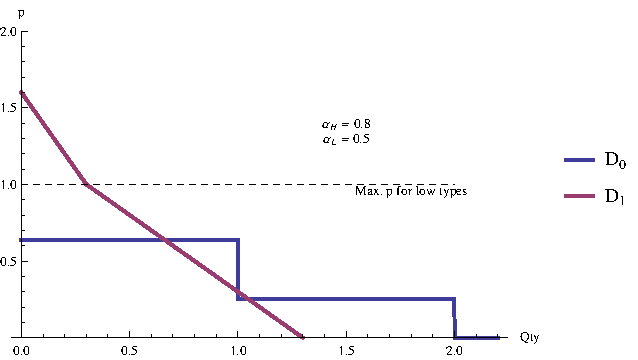
\includegraphics[scale = 1]{./diagrams/p2plr_demand.pdf}
%% \end{figure} 


%% Figure~\ref{fig:demand} shows this and it shows that with the P2P rental market in long-run equilibrium, demand can be non-zero above this point.  
%Intuitively, if a would-be owner can earn rental income from their unused capacity, it seems likely that a higher product market price is supportable. 

%% In this high-price range, the $D_1$ curve is kinked at $p = 2\alpha_L$. 
%% \important{The reason for this kink is that if $2\alpha_L < p$, the low-types do not use the good in the long-run P2P equilibrium.} 
%% The reason is simple: if $p > 2\alpha_L$, usage of the good offers negative utility from any amount of usage and so the low-types use none. 
